% .s1 manuscript, preprint (bioRxiv/arXiv) layout: plain single-column article with the same sections, figures and
% tables as the TCBB version (main.tex). Supplement and specification are the separate supplement.tex and spec.tex.
% Build after main.tex and supplement.tex (references to the supplement resolve through xr):
%   latexmk -pdf supplement.tex main.tex biorxiv.tex
\documentclass[11pt,letterpaper]{article}
\usepackage[margin=1in]{geometry}
\usepackage{newtxtext}
% Shared by main.tex (IEEEtran, the TCBB submission), supplement.tex and spec.tex: packages that work under both
% IEEEtran and article, the generated-number macros, house colours and pgfplots settings.
\usepackage[T1]{fontenc}
\usepackage{amsmath,amssymb}
\usepackage[scale=0.9]{plex-sans}   % figure text in IBM Plex, the singlet.bio typefaces
\usepackage[scale=0.86]{plex-mono}
\usepackage{microtype}
\usepackage{booktabs,tabularx,array}
\usepackage{xcolor}
\usepackage{graphicx}
\usepackage{tikz}
\usetikzlibrary{arrows.meta,positioning,fit,calc,decorations.pathreplacing,backgrounds}
\usepackage{pgfplots}
\usepackage{pgfplotstable}
\pgfplotsset{compat=1.18}
\usepgfplotslibrary{fillbetween}

% ---------- generated numbers ----------
\newcommand{\defnum}[2]{\expandafter\def\csname s1n@#1\endcsname{#2}}
\newcommand{\nm}[1]{\ifcsname s1n@#1\endcsname\csname s1n@#1\endcsname\else\textcolor{red!75!black}{\text{\sffamily\footnotesize[??\detokenize{#1}]}}\fi}
\InputIfFileExists{generated/numbers.tex}{}{}
\newcommand{\gen}[1]{generated/#1}   % path of a generated table

% ---------- house style ----------
\newcommand{\sone}{\texttt{.s1}}
% singlet.bio brand (singlet.bio/brand): teal for .s1, ink and grey-green neutrals, violet and amber accents
\definecolor{sone}{HTML}{0E8C7E}   % teal 500
\definecolor{gen}{HTML}{6B7C78}    % neutral, between muted and cell
\definecolor{dom}{HTML}{C2410C}
\definecolor{dl}{HTML}{B42318}     % limits: the floor of the count models
\definecolor{dec}{HTML}{B45309}    % amber: entropy coders, the output bound
\definecolor{tens}{HTML}{7C5CFF}   % violet: fitted trends
\definecolor{ink2}{HTML}{2B3F3C}   % ink 2
% One colour per storage format, the same in every panel that shows formats (Fig. 1 and the supplement). Families share
% a hue: HDF5 files orange to brown, Zarr greens, R files red, plain arrays grey; .s1 is the house blue. Colour names are
% c-<format id>, the ids of the `format` column of generated/*.tsv.
\definecolor{c-s1}{HTML}{2A78D6}
\definecolor{c-h5ad_none}{HTML}{F0B27A}
\definecolor{c-h5ad_lzf}{HTML}{E08A2E}
\definecolor{c-h5ad_gzip}{HTML}{B85A12}
\definecolor{c-tenx_h5}{HTML}{7A3B10}
\definecolor{c-loom}{HTML}{C9A26B}
\definecolor{c-zarr}{HTML}{55A868}
\definecolor{c-zarr3}{HTML}{2D6B40}
\definecolor{c-soma}{HTML}{8E6CC4}
\definecolor{c-bpcells}{HTML}{17A2B8}
\definecolor{c-parquet_coo}{HTML}{9AA33A}
\definecolor{c-mtx_gz}{HTML}{6E6E6E}
\definecolor{c-csc_i32}{HTML}{ABABAB}
\definecolor{c-csc_zstd19}{HTML}{D9B526}
\definecolor{c-rds_gz}{HTML}{D16B8F}
\definecolor{c-rds_xz}{HTML}{9E2F5E}
% every format but .s1, for loops over plots
\def\otherformats{h5ad_none,h5ad_lzf,h5ad_gzip,tenx_h5,loom,zarr,zarr3,soma,bpcells,parquet_coo,mtx_gz,csc_i32,csc_zstd19,rds_gz,rds_xz}

\emergencystretch=3em
\renewcommand{\topfraction}{0.95}\renewcommand{\textfraction}{0.05}\renewcommand{\floatpagefraction}{0.7}
\renewcommand{\dbltopfraction}{0.95}\renewcommand{\dblfloatpagefraction}{0.7}

% pgfplots: read tab-separated tables; keep only rows whose column #1 equals #2 (x or y filter)
\pgfplotsset{
  table/col sep=tab,
  discard if not/.style 2 args={x filter/.append code={\edef\tempa{\thisrow{#1}}\edef\tempb{#2}\ifx\tempa\tempb\else\def\pgfmathresult{nan}\fi}},
  discard if not y/.style 2 args={y filter/.append code={\edef\tempa{\thisrow{#1}}\edef\tempb{#2}\ifx\tempa\tempb\else\def\pgfmathresult{nan}\fi}},
  every axis/.append style={font=\sffamily\scriptsize, label style={font=\sffamily\scriptsize},
    axis line style={ink2!85}, every tick/.style={ink2!85},
    /pgf/number format/assume math mode=true,   % numbers in the figure font, not math digits
    tick label style={font=\sffamily\tiny}, title style={font=\sffamily\small\bfseries, align=left}},
}
\pgfplotstableset{col sep=tab, empty cells with={--}, every head row/.style={before row=\toprule, after row=\midrule},
  every last row/.style={after row=\bottomrule}}

\newcommand{\placeholder}[1]{\textcolor{red!75!black}{[#1]}}   % text still to be supplied by the author

\usepackage{caption}
\captionsetup{font=small,labelfont=bf}
\usepackage[nocompress]{cite}
\usepackage{xr-hyper}
\usepackage[colorlinks=true,linkcolor=blue!50!black,citecolor=blue!50!black,urlcolor=blue!50!black]{hyperref}
\externaldocument[S-]{supplement}   % supplement labels as S-<label>
\newcommand{\IEEEPARstart}[2]{#1#2}   % the sections are shared with the IEEEtran version
\newcommand{\para}[1]{\par\smallskip\noindent\textbf{#1.}\ }

\title{\sone: single-cell count matrices at the speed of the network}
\author{Zachary J.\ DeBruine\\[2pt]
  \small Department of Information Sciences and Technology, College of Computing, Grand Valley State University,
  Allendale, MI, USA\\
  \small Correspondence: \href{mailto:zacharydebruine@gmail.com}{zacharydebruine@gmail.com}}
\date{}

\begin{document}
\maketitle

\begin{abstract}
Moving data, not computing on them, now limits large single-cell analyses and model training. We measured how few bits
single-cell counts need and how fast integer codes decode, and used these limits to develop, with an AI coding assistant, a
format that approaches both. The format, \sone, models the counts with a static, context-conditioned entropy coder and reads
any subset of cells remotely. Across \nm{nMatrices} public matrices from \nm{nProtocolClasses} protocol classes, \sone{}
files were the smallest on every matrix, \nm{ratio-h5ad_gzip} times smaller than compressed AnnData and within a few
percent of the best count models. No measured code was both as small and faster to decode, and \sone{} decoded at the rate
the trend of existing codes predicts for its size. From cloud storage, \sone{} delivered a first minibatch in under a second
and streamed cells tens of times faster than chunked alternatives. Its costs are a decoder slower per core than
byte-oriented codes and a writer that needs more memory. We propose \sone{} as a standard format for single-cell counts.
\end{abstract}

% Introduction (main text). Numbers belong in the figures and their captions; the text states what they show.
\section{Introduction}
\label{sec:intro}

\IEEEPARstart{S}{ingle-cell} studies now routinely profile hundreds of thousands to millions of cells, reference atlases
hold tens of millions~\cite{svensson2018exponential,sikkema2023integrated,czi2025cellxgene}, and a single perturbation
screen has reached a hundred million~\cite{zhang2025tahoe}. These data are no longer analysed once on a laptop. Atlases
serve them to thousands of users, and machine-learning models stream them minibatch by minibatch, reading every cell many
times~\cite{lopez2018deep,theodoris2023transfer,cui2024scgpt}. More and more often they live in cloud object storage and
cross a network before they are used. Moving the data, rather than computing on them, has become a bottleneck for
large-scale analysis and for building AI-ready datasets.

For a link of a given bandwidth, the number of cells delivered per second is set by how many bits each cell takes. That
number has a floor, the information the counts actually contain, and the formats in use stay far above it.
AnnData~\cite{virshup2024anndata}, the 10x Genomics HDF5 file, loom, Zarr and TileDB-SOMA~\cite{tiledbsoma} store a
matrix of whole-number counts as generic arrays and compress them with tools such as gzip or zstd, which see only bytes.
What limits how fast single-cell data can be delivered today is therefore mostly how they are encoded, not the network.

Count matrices are far from arbitrary. Most non-zero counts are exactly one; how deeply a cell was sequenced sets the
expected count of every gene in it; and if genes are numbered from most to least frequently detected, the positions of a
cell's non-zero entries become a short list of small steps. A code that knows these regularities can describe the same
matrix in far fewer bits, as domain-specific formats for sequencing reads did when they replaced gzip with models of their
data~\cite{bonfield2022cram}. But fewer bits help only if they can be decoded as fast as the link delivers them. Two
limits therefore matter together: how few bits a lossless code can spend on the counts, and how fast a code that small can
be decoded.

We measured both limits on real data and built a format that approaches them. The result is \sone, an open format for
single-cell count matrices, read and written from Python, R and C++ by the \texttt{singlet} package. Fig.~\ref{fig:wow}
summarises the outcome. This paper makes four contributions:
\begin{itemize}
\item \emph{Limits.} We estimate the information floor of \nm{nMatrices} public count matrices with cross-validated count
  models, and the speed frontier of the integer codes a format could adopt, each decoding the same matrices on one core
  (Section~\ref{sec:floor}).
\item \emph{A format.} \sone{} models the counts with a static, context-conditioned entropy coder, stores cells in
  independently decodable blocks behind an index, and names every file by its content (Section~\ref{sec:format}).
\item \emph{A benchmark.} We compare \sone{} with fifteen storage formats and settings on matrices from
  \nm{nProtocolClasses} protocol classes, from cold reads to training loaders on emulated and real cloud storage, with
  every number produced by one open pipeline (Section~\ref{sec:setup}).
\item \emph{Findings.} \sone{} files are the smallest on every matrix and within a few percent of the best count models; no
  measured code was both as small and faster to decode; and from cloud storage \sone{} keeps a network link busy where
  chunked formats leave it idle (Section~\ref{sec:results}). We also report its costs.
\end{itemize}
The codec was developed iteratively with an AI model, Claude (Anthropic), as a coding assistant, with every candidate
change measured against the limits above.

% Figure 1: the headline. Every value is read from generated/fig1*.tsv and generated/fig1a_boxes.tex (written by
% `python -m s1bench report`). One tikzpicture with the axes placed on a grid, so that panels share edges: a and b are
% square and side by side, c (two axes) sits under a and d under b, with the same height.
% \figbox{pos}{q1}{median}{q3}{low whisker}{high whisker}{colour}: one horizontal box of panel a, in axis coordinates.
\newcommand{\figbox}[7]{%
  \draw[#7!80!black, line width=0.5pt] (axis cs:#5,#1) -- (axis cs:#2,#1);
  \draw[#7!80!black, line width=0.5pt] (axis cs:#4,#1) -- (axis cs:#6,#1);
  \draw[#7!80!black, fill=#7, fill opacity=0.18, line width=0.5pt] (axis cs:#2,{#1-0.32}) rectangle (axis cs:#4,{#1+0.32});
  \draw[#7!70!black, line width=1.2pt] (axis cs:#3,{#1-0.32}) -- (axis cs:#3,{#1+0.32});}
% an axis break across a bar that leaves the scale: two slanted strokes on a white gap at (#1, row #2) in axis units
\newcommand{\figbreak}[2]{%
  \fill[white] ($(axis cs:#1,{#2-0.34})+(-1.5pt,0)$) rectangle ($(axis cs:#1,{#2+0.34})+(1.5pt,0)$);
  \draw[ink2, line width=0.5pt] ($(axis cs:#1,{#2+0.34})+(-3pt,0)$) -- ($(axis cs:#1,{#2-0.34})+(0pt,0)$);
  \draw[ink2, line width=0.5pt] ($(axis cs:#1,{#2+0.34})+(0pt,0)$) -- ($(axis cs:#1,{#2-0.34})+(3pt,0)$);
}
\begin{figure*}[tbp]
\centering
\pgfmathsetlengthmacro{\figS}{0.34\linewidth}      % side of the square panels a and b
\pgfmathsetlengthmacro{\figH}{0.52*\figS}          % height of panels c and d
\pgfmathsetlengthmacro{\figG}{1.75cm}              % horizontal gap: the y label and tick labels of b and d
\pgfmathsetlengthmacro{\figV}{1.45cm}              % vertical gap: the x labels of a and b and the titles of c and d
\pgfmathsetlengthmacro{\figCw}{0.46*\figS}         % width of each half of panel c
\begin{tikzpicture}
% ---------------- (a) compression ratio of every matrix against uncompressed CSC ----------------
\begin{axis}[name=pa, at={(0,0)}, anchor=north west, scale only axis, width=\figS, height=\figS,
  title={a\quad Compression of every matrix},
  xmin=0, xmax=17, xtick={0,2,...,16}, xlabel={compression ratio against 32-bit CSC arrays ($\times$)},
  ytick=data, ytick style={draw=none}, yticklabels from table={\gen{fig1a_size.tsv}}{label}, y dir=reverse, enlarge y limits=0.04,
  axis x line*=bottom, axis y line*=left, clip=false]
\addplot[draw=none, forget plot] table[x=ratio_median, y=pos] {\gen{fig1a_size.tsv}};   % sets the y ticks
\draw[gen!60, line width=0.4pt, dashed] (axis cs:1,-0.5) -- (axis cs:1,15.5);
\input{\gen{fig1a_boxes.tex}}
\expandafter\pgfplotsinvokeforeach\expandafter{\otherformats,s1}{
  \addplot[only marks, mark=*, mark size=0.75pt, c-#1, opacity=0.6, discard if not={format}{#1}] table[x=ratio, y=y] {\gen{fig1a_points.tsv}};
}
\end{axis}
% ---------------- (b) size vs speed with R_eff iso-lines (figures/fig1b_panel.tex) ----------------
\def\fbLog{0}\def\fbPts{1}\def\fbTitle{b\quad Smaller and faster, four cores}\def\fbInPicture{1}
\def\fbAxisOpts{name=pb, at={($(pa.north east)+(\figG,0)$)}, anchor=north west, scale only axis, width=\figS, height=\figS}
% Fig. 1b: stored size against cold read rate, from generated/fig1c_tradeoff.tsv (medians and quartiles per format) and
% generated/fig1b_points.tsv (every matrix). Set before \input: \def\fbLog{1} for log axes or {0} for linear ones, and
% \def\fbPts{1} to draw every matrix (with \def\fbPts{0} each median gets its interquartile ranges instead), and the
% panel title in \fbTitle.
\ifnum\fbLog=1
  \def\fbopts{xmode=log, ymode=log, xmin=3, xmax=110, ymin=2, ymax=2000,
    xtick={5,10,20,50,100}, xticklabels={5,10,20,50,100}, ytick={10,100,1000}, yticklabels={10,100,1000},
    xlabel={stored bits per non-zero (log scale)}, ylabel={cold read rate, million non-zeros/s (log scale)}}
  \def\fbiso{25,50,100,200}\def\fbxlo{3}\def\fbtop{1500}\def\fbanchor{anchor}
\else
  \def\fbopts{xmin=0, xmax=70, ymin=0, ymax=260, xtick={0,10,...,70}, ytick={0,50,...,250},
    xlabel={stored bits per non-zero}, ylabel={cold read rate, million non-zeros/s}}
  \def\fbiso{25,50,100}\def\fbxlo{0.2}\def\fbtop{250}\def\fbanchor{anchor_lin}
\fi
% Inside another tikzpicture (Fig. 1), \fbAxisOpts gives the axis position and size and no picture is opened here.
\def\fbaxis#1{\begin{axis}[#1]}
\ifdefined\fbAxisOpts\else\begin{tikzpicture}\def\fbAxisOpts{width=0.47\linewidth, height=7.6cm}\fi
\edef\fbAll{\unexpanded\expandafter{\fbopts},\unexpanded\expandafter{\fbAxisOpts}}
\expandafter\fbaxis\expandafter{\fbAll,
  title={\fbTitle}, clip mode=individual,
  axis x line*=bottom, axis y line*=left,
  lbl/.style={nodes near coords, point meta=explicit symbolic, visualization depends on={value \thisrow{\fbanchor}\as\lblanchor},
    every node near coord/.append style={font=\sffamily\tiny, anchor=\lblanchor, text=ink2, inner sep=1.5pt}},
  iqr/.style={error bars/x dir=both, error bars/y dir=both, error bars/x explicit, error bars/y explicit,
    error bars/error bar style={line width=0.5pt, opacity=0.8}, error bars/error mark=none},
}
% iso-lines of Eq. (1) at B = 1 Gbit/s: R_eff = R  <=>  D = 1/(1/R - b/1000), D and R in million non-zeros/s, b in bits;
% each ends, labelled, at the top of the plot
\expandafter\pgfplotsinvokeforeach\expandafter{\fbiso}{
  \addplot[domain=\fbxlo:{1000*(1/#1-1/\fbtop)}, samples=150, dashed, sone!55, forget plot] {1/(1/#1 - x/1000)}
    node[pos=1, anchor=south west, font=\sffamily\tiny, text=sone!80!black, inner sep=1pt] {#1\,M/s};
}
\node[anchor=north east, font=\sffamily\tiny, text=sone!80!black, align=right, inner sep=1pt] at (rel axis cs:0.99,0.89)
  {dashed: non-zeros per second\\delivered over a 1\,Gbit/s link};
% labels: beside each median on log axes; on linear axes beside, above or below each point, placed by
% generated/fig1d_labels.tex to avoid overlaps
\tikzset{fblabel/.style={font=\sffamily\tiny, text=ink2, inner sep=0.6pt, outer sep=0pt, fill=white, fill opacity=0.8, text opacity=1}}
\ifnum\fbLog=1\pgfplotsset{fblbl/.style={lbl}}\else\pgfplotsset{fblbl/.style={}}\input{\gen{fig1d_labels.tex}}\fi
\ifnum\fbPts=1
\expandafter\pgfplotsinvokeforeach\expandafter{\otherformats,s1}{
  \addplot[only marks, mark=*, mark size=0.7pt, c-#1, opacity=0.4, forget plot, discard if not={format}{#1}] table[x=bits, y=mnnzs] {\gen{fig1b_points.tsv}};
}
\pgfplotsset{fbmed/.style={draw=white, line width=0.4pt}}
\else
\pgfplotsset{fbmed/.style={iqr}}
\fi
\expandafter\pgfplotsinvokeforeach\expandafter{\otherformats}{
\addplot[only marks, fblbl, mark=*, mark size=1.8pt, c-#1, fbmed, discard if not={format}{#1}]
  table[x=bits, y=mnnzs, meta=label, x error plus expr=\thisrow{bits_q3}-\thisrow{bits}, x error minus expr=\thisrow{bits}-\thisrow{bits_q1},
    y error plus expr=\thisrow{mnnzs_q3}-\thisrow{mnnzs}, y error minus expr=\thisrow{mnnzs}-\thisrow{mnnzs_q1}] {\gen{fig1c_tradeoff.tsv}};
}
\addplot[only marks, fblbl, mark=*, mark size=2.4pt, c-s1, fbmed, discard if not={format}{s1}]
  table[x=bits, y=mnnzs, meta=label, x error plus expr=\thisrow{bits_q3}-\thisrow{bits}, x error minus expr=\thisrow{bits}-\thisrow{bits_q1},
    y error plus expr=\thisrow{mnnzs_q3}-\thisrow{mnnzs}, y error minus expr=\thisrow{mnnzs}-\thisrow{mnnzs_q1}] {\gen{fig1c_tradeoff.tsv}};
\end{axis}
\ifdefined\fbInPicture\else\end{tikzpicture}\let\fbAxisOpts\undefined\fi%

% ---------------- (c) time to the first minibatch, then per minibatch ----------------
% Bars fill half of each row (bar width 0.5 in axis units, rows 1 apart), so gaps equal bars. TileDB-SOMA ML leaves both
% scales: its bar is cut by an axis break and labelled inside with its value.
\pgfplotsset{fig1c/.style={xbar, bar shift=0pt, bar width=0.5, ymin=-0.5, ymax=3.5, y dir=reverse,
  scale only axis, width=\figCw, height=\figH, axis x line*=bottom, axis y line*=left, clip=false,
  ytick={0,1,2,3}, ytick style={draw=none}},
  fig1cval/.style={nodes near coords style={font=\sffamily\tiny, anchor=west, text=ink2}},
  fig1cin/.style={nodes near coords style={font=\sffamily\tiny, anchor=east, text=white}}}
\begin{axis}[fig1c, name=pc, at={($(pa.south west)+(0,-\figV)$)}, anchor=north west,
  title={c\quad First minibatch\ldots}, xmin=0, xmax=0.5, xtick={0,0.2,0.4}, xlabel={seconds},
  yticklabels from table={\gen{fig1b_ttfm.tsv}}{label},
  point meta=explicit, nodes near coords={\pgfmathprintnumber[fixed, fixed zerofill, precision=2, assume math mode=true]{\pgfplotspointmeta}\,s}]
\pgfplotsinvokeforeach{s1,zarr3,zarr}{
  \addplot[fill=c-#1, draw=none, fig1cval, discard if not y={fmt}{#1}] table[x=total, y=pos, meta=total] {\gen{fig1b_ttfm.tsv}};
}
\addplot[fill=c-soma, draw=none, fig1cin, discard if not y={fmt}{soma}] table[x expr={0.5}, y=pos, meta=total] {\gen{fig1b_ttfm.tsv}};
\figbreak{0.33}{3}
\end{axis}
\begin{axis}[fig1c, name=pc2, at={($(pc.north east)+(0.08*\figS,0)$)}, anchor=north west,
  title={\ldots then each minibatch}, xmin=0, xmax=400, xtick={0,200,400}, xlabel={milliseconds}, yticklabels={},
  point meta=explicit, nodes near coords={\pgfmathprintnumber[fixed, precision=0, assume math mode=true]{\pgfplotspointmeta}\,ms}]
\pgfplotsinvokeforeach{s1,zarr3,zarr}{
  \addplot[fill=c-#1, draw=none, fig1cval, discard if not y={fmt}{#1}] table[x expr={1000*\thisrow{per_batch}}, y=pos, meta expr={1000*\thisrow{per_batch}}] {\gen{fig1b_ttfm.tsv}};
}
\addplot[fill=c-soma, draw=none, fig1cin, discard if not y={fmt}{soma}] table[x expr={400}, y=pos, meta expr={1000*\thisrow{per_batch}}] {\gen{fig1b_ttfm.tsv}};
\figbreak{260}{3}
\end{axis}
% ---------------- (d) speed-up over one core, formats that decode in parallel ----------------
\begin{axis}[name=pd, at={($(pb.south west)+(0,-\figV)$)}, anchor=north west, scale only axis, width=\figS, height=\figH,
  title={d\quad Parallel decoding},
  xmode=log, log basis x=2, ymode=log, log basis y=2, xmin=0.85, xmax=9.5, ymin=0.9, ymax=9,
  xtick={1,2,4,8}, xticklabels={1,2,4,8}, ytick={1,2,4,8}, yticklabels={1$\times$,2$\times$,4$\times$,8$\times$},
  xlabel={cores}, ylabel={read rate $\div$ one core},
  axis x line*=bottom, axis y line*=left, unbounded coords=jump,
  legend style={font=\sffamily\tiny, draw=none, fill=none, at={(0.02,0.98)}, anchor=north west, legend columns=1, cells={anchor=west}}]
\addplot[gen!70, densely dotted, no marks, forget plot] table[x=threads, y=ideal] {\gen{fig1d_speedup.tsv}}
  node[pos=0.55, sloped, above, font=\sffamily\tiny, text=gen] {ideal};
\addplot[c-s1, very thick, mark=*, mark size=1.6pt] table[x=threads, y=s1] {\gen{fig1d_speedup.tsv}};
\addplot[c-soma, thick, mark=triangle*, mark size=1.5pt] table[x=threads, y=soma] {\gen{fig1d_speedup.tsv}};
\addplot[c-mtx_gz, thick, mark=square*, mark size=1.2pt] table[x=threads, y=mtx_gz] {\gen{fig1d_speedup.tsv}};
\addplot[c-parquet_coo, thick, mark=diamond*, mark size=1.5pt] table[x=threads, y=parquet_coo] {\gen{fig1d_speedup.tsv}};
\addplot[c-zarr3, thick, mark=pentagon*, mark size=1.4pt] table[x=threads, y=zarr3] {\gen{fig1d_speedup.tsv}};
\legend{\sone, TileDB-SOMA, MTX.gz, Parquet COO, {Zarr v3, sharded}}
\end{axis}
\end{tikzpicture}
\caption{\textbf{\sone{} files are the smallest on every matrix and, on four cores, the fastest to read on
\nm{dec-s1-fastest-count} of \nm{dec-paired-n}.}
\textbf{(a)} Compression ratio of each format's file (counts, gene identifiers and barcodes) against uncompressed CSC
arrays with 32-bit indices and values, one point per matrix (\nm{nMatrices} matrices); boxes, quartiles and median;
whiskers, the most extreme matrices within 1.5 interquartile ranges. \sone{} compresses a median of \nm{cr-s1}$\times$
(\nm{cr-s1-lo}--\nm{cr-s1-hi}$\times$), gzip-compressed AnnData \nm{cr-h5ad_gzip}$\times$.
\textbf{(b)} Size against read rate from a cold file into an in-memory sparse matrix on \nm{threadsHeadline} cores: one
faint point per matrix and format, large points the medians. Dashed lines join sizes and decode rates that deliver the same
number of non-zeros per second over a 1\,Gbit/s link (Eq.~\ref{eq:reff}); up and to the left is better. On one core
\sone{} reads \nm{dec-s1-t1} million non-zeros per second, behind uncompressed arrays (Table~\ref{tab:main}). Log axes:
Supplementary Fig.~\ref{S-fig:sfig1b}.
\textbf{(c)} Seconds from a new process to the first 512-cell training minibatch, decoded into a PyTorch sparse tensor,
and milliseconds per minibatch after that; \nm{fig1b-dataset} read from an object store over a \nm{fig1b-tier} link,
median of three seeds. Bars cut by an axis break carry their value inside. Loaders that download the whole file first are
in Supplementary Table~\ref{S-tab:minibatch}.
\textbf{(d)} Read rate from a cold file relative to one core, median of per-matrix ratios, for the \nm{par-formats-n} of
\nm{par-formats-of} formats whose readers use more than one core.}
\label{fig:wow}
\end{figure*}


% Related work (main text): prior work only; results of this paper are in results.tex.
\section{Related work}
\label{sec:related}

\para{Storing count matrices}On disk, almost every single-cell toolkit stores the compressed sparse column (CSC) layout of
its in-memory matrices~\cite{bates2024matrix,virtanen2020scipy}: 32-bit row indices and 32- or 64-bit values, 64 to 96
bits per non-zero, however small the counts are. Matrix Market~\cite{boisvert1997matrix} writes them as text; the 10x HDF5
file~\cite{zheng2017massively,tenx_h5}, loom~\cite{loompy} and AnnData~\cite{virshup2024anndata} (in HDF5~\cite{hdf5} or
Zarr~\cite{zarr}) store chunked arrays, compressed by byte-level filters such as gzip, LZF, Blosc or
zstd~\cite{deutsch1996deflate,collet2021zstd}. Formats built for scale add structure: TileDB-SOMA~\cite{papadopoulos2016tiledb,tiledbsoma}
serves the CELLxGENE Census~\cite{czi2025cellxgene}, BPCells~\cite{parks2025bpcells} bit-packs deltas and values for
streaming reads, and Parquet~\cite{parquet} distributes the largest training corpora~\cite{tahoe100m_hf}. Our earlier VCSC
and IVCSC layouts store each distinct value of a column once and delta-encode and byte-pack its row indices, shrinking
single-cell matrices several-fold below CSC in memory~\cite{ruiter2024vcsc}. None of these uses an entropy coder with a
model of the counts.

\para{Compressing integers}Inverted indexes face the same problem as CSC row indices: sorted integer lists with small gaps.
Byte- and bit-aligned codes~\cite{lemire2018stream,lemire2015decoding} decode billions of integers per second because they
ignore the distribution of the values; entropy coders spend close to $-\log_2 p$ bits per symbol~\cite{cover2006elements}
at a higher cost per symbol. Asymmetric numeral systems~\cite{duda2013asymmetric} with interleaved states decode several
symbols at once on SIMD units~\cite{giesen2014interleaved}, and ANS with contexts closes much of the gap between fast and
small codes for inverted indexes~\cite{moffat2017ans,moffat2020large,pibiri2021techniques}, the closest precedent for
\sone.

\para{Models of genomic data}CRAM~3.1 replaced BAM's gzip blocks with per-field models and 32-way interleaved
rANS~\cite{bonfield2022cram}; benchmarks of read compressors found that how each field is modelled matters more than the
back-end coder~\cite{numanagic2016comparison,hernaez2019genomic}, and genotype matrices have compressors of their
own~\cite{danek2018gtc,lan2021genozip}. For counts, UMI data are close to Poisson samples of a cell's molecules given its
depth~\cite{townes2019feature,kim2020demystifying}, with a negative binomial for biological
variation~\cite{svensson2020droplet,hafemeister2019normalization} and heavy-tailed expression across
genes~\cite{furusawa2003zipf}. These models say what a coder can exploit, and which bits no lossless code can remove.

\para{Feeding models}Training draws random minibatches of cells many times over. scDataset fetches blocks of contiguous
cells and shuffles them in a buffer~\cite{dascenzo2025scdataset}, the Census provides a loader over
TileDB-SOMA~\cite{tiledbsomaml}, and cloud-native formats such as Zarr cut round trips, each of which waits tens of
milliseconds, with independently addressable chunks~\cite{abernathey2021cloud,durner2023exploiting}. These loaders
optimise access over existing encodings; \sone{} changes the encoding.

% The .s1 format (main text). The normative specification is a separate supplementary file (spec.tex).
\section{The \sone{} format}
\label{sec:format}\label{sec:how}

Fig.~\ref{fig:how} shows the format from a whole dataset down to individual bits; the full specification is a separate
supplementary file. A dataset is a small manifest that lists one file per sample, each named by a cryptographic hash of
its contents, so a link always refers to exactly the same bytes and anyone can check them (Fig.~\ref{fig:how}a).
Information shared by many samples, such as the gene names of a genome annotation, is stored once and downloaded once
(Fig.~\ref{fig:how}b). Table~\ref{tab:props} compares these properties with those of other formats.

\para{Blocks for partial reads}How does a reader get a few hundred cells out of a remote file without reading the rest?
Each count matrix starts with a small index that says where every block of consecutive cells lives in the file, and each
block decodes on its own (Fig.~\ref{fig:how}c). A reader fetches the index once and then only the blocks it needs, with one
request per run of blocks, from a local disk, a web server or a cloud bucket alike. Because every block is located before
any is read, all the requests of a minibatch can be sent at once.

\para{A model of the counts}Inside a block, genes are numbered from most to least frequently detected, so each cell's
non-zero entries become a sequence of small steps and small counts, most of them ones. Each entry becomes one short
symbol, and its probability is looked up in a table chosen by two things the reader already knows: how many entries the
cell has, and how far along the gene list it is (Fig.~\ref{fig:how}d). An rANS entropy coder~\cite{duda2013asymmetric}
then spends close to the minimum number of bits on each symbol. The tables are fixed for the whole matrix, so decoding is
a few table look-ups per entry, and 32 coders run side by side so that a processor with AVX2 decodes eight to sixteen
symbols at once. Writing a file ends with a full decode that must reproduce the input exactly.

% Figure 2: how .s1 stores single-cell counts, as four panels joined by zoom wedges, lettered as sections/format.tex
% cites them: (a) a dataset, (b) one sample file (header, member table, shared packs), (c) one count-matrix member
% (prefix, chunks, range requests), (d) one chunk. Plain words stand in for spec terms: "table of contents" is the
% member table, "block" a chunk, "code tables" the entropy tables, "gene order" the row keys, "symbol" the gap symbol
% (sigma, amber: the residual rho), "coders" the rANS lanes. Sizes, the prefix, the request pattern, the 12 x 40
% contexts (ctx_kind 0) and the chunk byte order follow sections/supplement_spec.tex. Genes, counts and ranks in (d)
% are a worked example of those rules, not data. Request labels in (c) follow the reference client
% (python/singlet/s1/client.py: the first request carries the prefix, then one request per run of chunks).
\begin{figure*}[tbp]
\centering
% panel title with a hanging indent after the panel letter
\def\ptitle#1#2#3#4{\node[ptit, text width=#3] at (#1) {\hyphenpenalty=10000\exhyphenpenalty=10000\hangindent=0.36cm\hangafter=1\makebox[0.36cm][l]{\small #2}#4};}
% station title in panel d
\def\stitle#1#2#3#4{\node[stit, text width=#2] at (#1) {\hyphenpenalty=10000\exhyphenpenalty=10000\hangindent=0.28cm\hangafter=1\makebox[0.28cm][l]{\bfseries #3}#4};}
% zoom wedge from a parent element's corners (#1, #2) to a child panel's corners (#3, #4)
\def\zoomwedge#1#2#3#4{\begin{scope}[on background layer]\fill[sone!5] (#1)--(#3)--(#4)--(#2)--cycle;\draw[wl] (#1)--(#3) (#2)--(#4);\end{scope}}
% one row of the table of contents in (b): y, style, name, start, length
\def\tocrow#1#2#3#4#5{%
  \node[cell,#2,minimum width=1.95cm,anchor=north west] at (6.75,#1) {#3};
  \node[cell,#2,minimum width=0.80cm,anchor=north west,align=center] at (8.70,#1) {#4};
  \node[cell,#2,minimum width=0.80cm,anchor=north west,align=center] at (9.50,#1) {#5};}
% legend chips for the note in (d): blue symbol, amber symbol
\def\chipkey#1#2{{\setlength{\fboxsep}{0pt}\fcolorbox{#1}{#2}{\rule{0pt}{5.5pt}\hspace{8pt}}}}
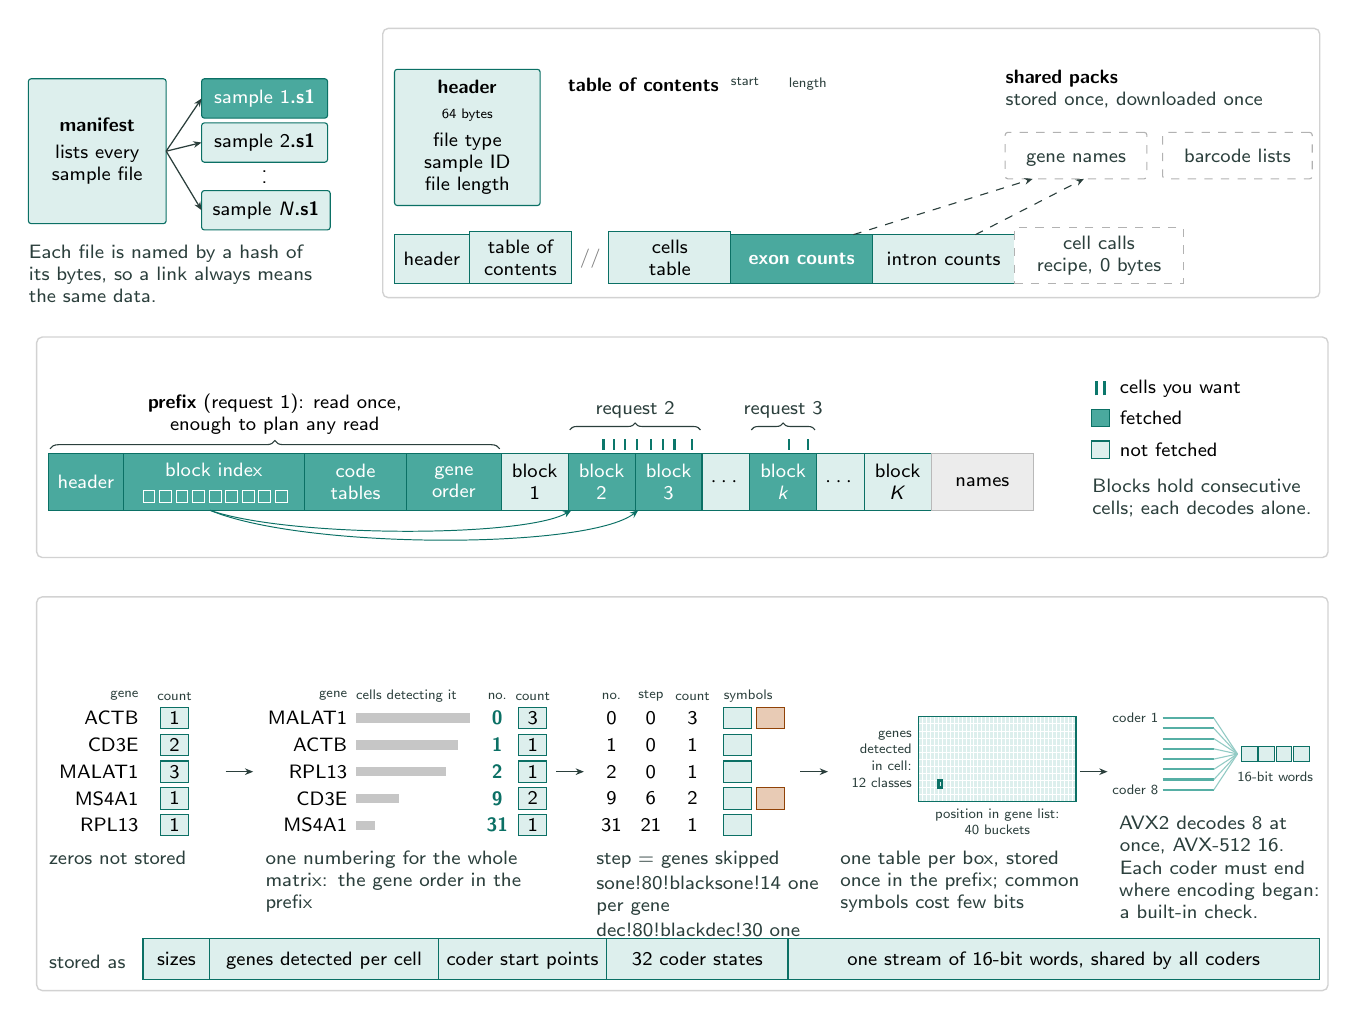
\begin{tikzpicture}[
  x=1cm, y=1cm,
  font=\sffamily\scriptsize,
  >={Stealth[length=3pt,width=2.4pt]},
  st/.style={draw=sone!80!black, fill=sone!14, line width=0.4pt},
  hot/.style={draw=sone!80!black, fill=sone!75, text=white, line width=0.4pt},
  idle/.style={draw=gray!55, fill=gray!15, line width=0.4pt},
  ghost/.style={draw=gray!60, dashed, fill=white, text=ink2, line width=0.4pt},
  amb/.style={draw=dec!80!black, fill=dec!30, line width=0.4pt},
  seg/.style={rectangle, inner sep=3pt, outer sep=0pt, align=center, anchor=south west},
  box/.style={rectangle, inner sep=4pt, outer sep=0pt, align=center, rounded corners=1pt},
  cell/.style={rectangle, inner sep=3pt, outer sep=0pt, align=left, minimum height=0.36cm, text depth=0.5pt},
  frame/.style={draw=gray!35, rounded corners=2pt, line width=0.5pt},
  ptit/.style={font=\sffamily\scriptsize\bfseries, anchor=north west, inner sep=0pt, align=left},
  stit/.style={font=\sffamily\scriptsize, anchor=north west, inner sep=0pt, align=left},
  note/.style={text=ink2, inner sep=0pt, align=left},
  hd/.style={font=\sffamily\tiny, text=ink2, inner sep=0pt},
  wl/.style={draw=gray!55, line width=0.4pt},
  arr/.style={->, ink2, line width=0.45pt},
  chip/.style={rectangle, inner sep=0pt, outer sep=0pt, minimum height=0.27cm, minimum width=0.36cm, line width=0.4pt},
]

% =============================================================== (a) a dataset
\ptitle{0,0}{a}{4.1cm}{A dataset}
\node[box, st, anchor=north west, minimum width=1.75cm, minimum height=1.84cm] (man) at (0,-0.62)
  {\textbf{manifest}\\[2pt]lists every\\sample file};
\node[box, hot, anchor=north west, minimum width=1.6cm, minimum height=0.36cm] (s1) at (2.2,-0.62) {sample 1\textbf{.s1}};
\node[box, st,  anchor=north west, minimum width=1.6cm, minimum height=0.36cm] (s2) at (2.2,-1.18) {sample 2\textbf{.s1}};
\node at (3.0,-1.83) {$\vdots$};
\node[box, st,  anchor=north west, minimum width=1.6cm, minimum height=0.36cm] (sN) at (2.2,-2.04) {sample \textit{N}\textbf{.s1}};
\foreach \s in {s1,s2,sN} \draw[arr] (man.east) -- (\s.west);
\node[note, anchor=north west, text width=3.75cm] at (0,-2.72)
  {Each file is named by a hash of its bytes, so a link always means the same data.};

% =============================================================== (b) one sample file
\draw[frame] (4.5,0.02) rectangle (16.4,-3.4);
\ptitle{4.62,-0.08}{b}{6cm}{One sample file}
% the file as stored
\node[seg, st,  minimum width=0.95cm, minimum height=0.62cm] (hdrB) at (4.65,-3.22) {header};
\node[seg, st,  minimum width=1.30cm, minimum height=0.62cm] (tocB) at (hdrB.south east) {table of\\contents};
\node[seg,      minimum width=0.40cm, minimum height=0.62cm, text=gray] (brkB) at (tocB.south east) {//};
\node[seg, st,  minimum width=1.55cm, minimum height=0.62cm] (celB) at (brkB.south east) {cells\\table};
\node[seg, hot, minimum width=1.80cm, minimum height=0.62cm] (cntB) at (celB.south east) {\textbf{exon counts}};
\node[seg, st,  minimum width=1.80cm, minimum height=0.62cm] (intB) at (cntB.south east) {intron counts};
\node[seg, ghost, minimum width=2.15cm, minimum height=0.62cm] (derB) at (intB.south east) {cell calls\\recipe, 0 bytes};
% zoom: header and table of contents
\node[box, st, anchor=north west, minimum width=1.85cm, minimum height=1.66cm] (hdrZ) at (4.65,-0.5)
  {\textbf{header}\\[1pt]{\tiny 64 bytes}\\[2pt]file type\\sample ID\\file length};
\node[cell, anchor=north west, minimum width=1.95cm, font=\sffamily\scriptsize\bfseries] at (6.75,-0.5) {table of contents};
\node[hd, anchor=north] at (9.10,-0.6) {start};
\node[hd, anchor=north] at (9.90,-0.6) {length};
\tocrow{-0.83}{st}{cells}{\textit{o}\textsubscript{1}}{\textit{l}\textsubscript{1}}
\tocrow{-1.19}{hot}{exon counts}{\textit{o}\textsubscript{2}}{\textit{l}\textsubscript{2}}
\tocrow{-1.55}{st}{intron counts}{\textit{o}\textsubscript{3}}{\textit{l}\textsubscript{3}}
\tocrow{-1.91}{ghost}{cell calls}{0}{0}
\zoomwedge{hdrB.north west}{tocB.north east}{4.65,-2.24}{10.3,-2.24}
% shared packs
\node[note, anchor=north west, text width=3.8cm, text=black] at (12.3,-0.5)
  {\textbf{shared packs}\\\textcolor{ink2}{stored once, downloaded once}};
\node[box, ghost, anchor=north west, minimum width=1.8cm, minimum height=0.5cm, text height=1.6ex, text depth=0.45ex] (pkG) at (12.3,-1.3) {gene names};
\node[box, ghost, anchor=north west, minimum width=1.9cm, minimum height=0.5cm, text height=1.6ex, text depth=0.45ex] (pkB) at (14.3,-1.3) {barcode lists};
\draw[->, dashed, ink2, line width=0.4pt] ($(cntB.north east)+(-0.35,0)$) -- ($(pkG.south west)+(0.35,0)$);
\draw[->, dashed, ink2, line width=0.4pt] ($(intB.north)+(0.3,0)$) -- ($(pkG.south)+(0.1,0)$);

% =============================================================== (c) one count matrix
\draw[frame] (0,-3.9) rectangle (16.4,-6.7);
\ptitle{0.12,-4.0}{c}{12cm}{One count matrix: a small prefix, then blocks of cells}
\node[seg, hot, minimum width=0.95cm, minimum height=0.72cm] (hdrC) at (0.15,-6.1) {header};
\node[seg, hot, minimum width=2.30cm, minimum height=0.72cm] (idxC) at (hdrC.south east) {};
\node[text=white, inner sep=0pt] at ($(idxC.north)+(0,-0.2)$) {block index};
\foreach \i in {0,...,8} \draw[white, line width=0.3pt] ($(idxC.south west)+(0.25+0.21*\i,0.1)$) rectangle ++(0.15,0.15);
\node[seg, hot, minimum width=1.30cm, minimum height=0.72cm] (tabC) at (idxC.south east) {code\\tables};
\node[seg, hot, minimum width=1.20cm, minimum height=0.72cm] (ordC) at (tabC.south east) {gene\\order};
\node[seg, st,  minimum width=0.85cm, minimum height=0.72cm] (b1) at (ordC.south east) {block\\1};
\node[seg, hot, minimum width=0.85cm, minimum height=0.72cm] (b2) at (b1.south east) {block\\2};
\node[seg, hot, minimum width=0.85cm, minimum height=0.72cm] (b3) at (b2.south east) {block\\3};
\node[seg, st,  minimum width=0.55cm, minimum height=0.72cm] (bd1) at (b3.south east) {$\cdots$};
\node[seg, hot, minimum width=0.85cm, minimum height=0.72cm] (bk) at (bd1.south east) {block\\\textit{k}};
\node[seg, st,  minimum width=0.55cm, minimum height=0.72cm] (bd2) at (bk.south east) {$\cdots$};
\node[seg, st,  minimum width=0.85cm, minimum height=0.72cm] (bK) at (bd2.south east) {block\\\textit{K}};
\node[seg, idle, minimum width=1.30cm, minimum height=0.72cm] (nmC) at (bK.south east) {names};
% the prefix
\draw[decorate, decoration={brace, amplitude=3pt}, ink2, line width=0.4pt] ($(hdrC.north west)+(0.02,0.06)$) -- ($(ordC.north east)+(-0.02,0.06)$)
  node[midway, above=5pt, note, align=center, text=black] {\textbf{prefix} (request 1): read once,\\enough to plan any read};
% the wanted cells and one request per run of blocks
\foreach \x in {7.20,7.33,7.47,7.62,7.80,7.95,8.10,8.32,9.55,9.80}
  \draw[sone!85!black, line width=0.8pt] (\x,-5.33) -- (\x,-5.19);
\draw[decorate, decoration={brace, amplitude=2.5pt}, ink2, line width=0.4pt] ($(b2.north west)+(0.02,0.3)$) -- ($(b3.north east)+(-0.02,0.3)$)
  node[midway, above=4pt, inner sep=0pt] {request 2};
\draw[decorate, decoration={brace, amplitude=2.5pt}, ink2, line width=0.4pt] ($(bk.north west)+(0.02,0.3)$) -- ($(bk.north east)+(-0.02,0.3)$)
  node[midway, above=4pt, inner sep=0pt] {request 3};
% index entries point at block starts
\draw[->, sone!80!black, line width=0.35pt] (2.2,-6.1) .. controls (3.2,-6.45) and (6.2,-6.45) .. ($(b2.south west)+(0.04,0)$);
\draw[->, sone!80!black, line width=0.35pt] (2.2,-6.1) .. controls (3.4,-6.6) and (7.0,-6.6) .. ($(b3.south west)+(0.04,0)$);
% legend
\draw[sone!85!black, line width=0.9pt] (13.46,-4.64) -- (13.46,-4.46) (13.56,-4.64) -- (13.56,-4.46);
\node[anchor=west, inner sep=0pt] at (13.75,-4.55) {cells you want};
\draw[hot] (13.4,-5.04) rectangle ++(0.22,0.22);
\node[anchor=west, inner sep=0pt] at (13.75,-4.93) {fetched};
\draw[st] (13.4,-5.44) rectangle ++(0.22,0.22);
\node[anchor=west, inner sep=0pt] at (13.75,-5.33) {not fetched};
\node[note, anchor=north west, text width=2.9cm] at (13.4,-5.7) {Blocks hold consecutive cells; each decodes alone.};

% =============================================================== (d) inside one block
\draw[frame] (0,-7.2) rectangle (16.4,-12.2);
\ptitle{0.12,-7.3}{d}{16cm}{Inside one block: each cell becomes small numbers, then short codes}
% --- station 1: one cell's counts
\stitle{0.15,-7.72}{2.3cm}{1}{One cell's counts}
\node[hd, anchor=east] at (1.3,-8.46) {gene};
\node[hd] at (1.75,-8.46) {count};
\foreach \g/\v [count=\i from 0] in {ACTB/1,CD3E/2,MALAT1/3,MS4A1/1,RPL13/1} {
  \node[anchor=east, inner sep=0pt] at (1.3,{-8.74-0.34*\i}) {\g};
  \node[chip, st] at (1.75,{-8.74-0.34*\i}) {\v};}
\node[note, anchor=north west] at (0.15,-10.42) {zeros not stored};
\draw[arr] (2.4,-9.42) -- (2.75,-9.42);
% --- station 2: genes numbered by detection
\stitle{2.9,-7.72}{3.6cm}{2}{Genes numbered, most often detected first}
\node[hd, anchor=east] at (3.95,-8.46) {gene};
\node[hd, anchor=west] at (4.05,-8.46) {cells detecting it};
\node[hd] at (5.85,-8.46) {no.};
\node[hd] at (6.3,-8.46) {count};
\foreach \g/\w/\d/\v [count=\i from 0] in {MALAT1/1.45/0/3,ACTB/1.3/1/1,RPL13/1.15/2/1,CD3E/0.55/9/2,MS4A1/0.25/31/1} {
  \node[anchor=east, inner sep=0pt] at (3.95,{-8.74-0.34*\i}) {\g};
  \fill[gray!45] (4.05,{-8.80-0.34*\i}) rectangle ++(\w,0.12);
  \node[font=\sffamily\scriptsize\bfseries, text=sone!80!black, inner sep=0pt] at (5.85,{-8.74-0.34*\i}) {\d};
  \node[chip, st] at (6.3,{-8.74-0.34*\i}) {\v};}
\node[note, anchor=north west, text width=3.6cm] at (2.9,-10.42) {one numbering for the whole matrix: the gene order in the prefix};
\draw[arr] (6.6,-9.42) -- (6.95,-9.42);
% --- station 3: steps and counts become symbols
\stitle{7.1,-7.72}{3.0cm}{3}{Small steps and small counts}
\node[hd] at (7.3,-8.46) {no.};
\node[hd] at (7.8,-8.46) {step};
\node[hd] at (8.33,-8.46) {count};
\node[hd, anchor=west] at (8.72,-8.46) {symbols};
\foreach \d/\s/\v/\two [count=\i from 0] in {0/0/3/1,1/0/1/0,2/0/1/0,9/6/2/1,31/21/1/0} {
  \node[inner sep=0pt] at (7.3,{-8.74-0.34*\i}) {\d};
  \node[inner sep=0pt] at (7.8,{-8.74-0.34*\i}) {\s};
  \node[inner sep=0pt] at (8.33,{-8.74-0.34*\i}) {\v};
  \node[chip, st, anchor=west] at (8.72,{-8.74-0.34*\i}) {};
  \ifnum\two=1 \node[chip, amb, anchor=west] at (9.14,{-8.74-0.34*\i}) {};\fi}
\node[note, anchor=north west, text width=3.0cm] at (7.1,-10.42)
  {step = genes skipped\\[1pt]
   \chipkey{sone!80!black}{sone!14}\ one per gene\\[1pt]
   \chipkey{dec!80!black}{dec!30}\ one more if count $\neq$\,1};
\draw[arr] (9.7,-9.42) -- (10.05,-9.42);
% --- station 4: a code table chosen by context
\stitle{10.2,-7.72}{3.0cm}{4}{Short codes for common symbols}
\begin{scope}[shift={(11.2,-9.8)}]
  \fill[sone!14] (0,0) rectangle (2.0,1.08);
  \draw[white, line width=0.15pt, xstep=0.05, ystep=0.09] (0,0) grid (2.0,1.08);
  \draw[sone!80!black, line width=0.4pt] (0,0) rectangle (2.0,1.08);
  \draw[sone!80!black, line width=0.9pt] (5*0.05,2*0.09) rectangle ++(0.05,0.09);
\end{scope}
\node[hd, align=right, anchor=east] at (11.12,-9.26) {genes\\detected\\in cell:\\12 classes};
\node[hd, anchor=north, align=center] at (12.2,-9.88) {position in gene list:\\40 buckets};
\node[note, anchor=north west, text width=3.1cm] at (10.2,-10.42)
  {one table per box, stored once in the prefix; common symbols cost few bits};
\draw[arr] (13.25,-9.42) -- (13.6,-9.42);
% --- station 5: 32 coders, one word stream
\stitle{13.75,-7.72}{2.55cm}{5}{32 rANS coders side by side (8 shown)}
\foreach \l in {0,...,7} {
  \draw[sone!70, line width=0.8pt] (14.3,{-8.74-0.13*\l}) -- (14.95,{-8.74-0.13*\l});
  \draw[sone!45, line width=0.4pt] (14.95,{-8.74-0.13*\l}) -- (15.25,-9.195);}
\node[hd, anchor=east] at (14.25,-8.74) {coder 1};
\node[hd, anchor=east] at (14.25,-9.65) {coder 8};
\foreach \w in {0,...,3} \draw[st] (15.3+0.22*\w,-9.295) rectangle ++(0.2,0.2);
\node[hd, anchor=north] at (15.73,-9.42) {16-bit words};
\node[note, anchor=north west, text width=2.55cm] at (13.75,-9.98)
  {AVX2 decodes 8 at once, AVX-512 16. Each coder must end where encoding began: a \mbox{built-in} check.};
% --- the block as stored
\node[anchor=west, inner sep=0pt, text=ink2] at (0.15,-11.83) {stored as};
\node[seg, st, minimum width=0.85cm, minimum height=0.46cm, text height=1.6ex, text depth=0.45ex] (f1) at (1.35,-12.06) {sizes};
\node[seg, st, minimum width=2.9cm, minimum height=0.46cm, text height=1.6ex, text depth=0.45ex] (f2) at (f1.south east) {genes detected per cell};
\node[seg, st, minimum width=2.1cm, minimum height=0.46cm, text height=1.6ex, text depth=0.45ex] (f3) at (f2.south east) {coder start points};
\node[seg, st, minimum width=2.3cm, minimum height=0.46cm, text height=1.6ex, text depth=0.45ex] (f4) at (f3.south east) {32 coder states};
\node[seg, st, minimum width=6.75cm, minimum height=0.46cm, text height=1.6ex, text depth=0.45ex] (f5) at (f4.south east) {one stream of 16-bit words, shared by all coders};

% =============================================================== zoom wedges
\zoomwedge{cntB.south west}{cntB.south east}{0,-3.9}{16.4,-3.9}
\zoomwedge{bk.south west}{bk.south east}{0,-7.2}{16.4,-7.2}
\zoomwedge{s1.north east}{s1.south east}{4.5,0.02}{4.5,-3.4}
\end{tikzpicture}
\caption{\textbf{How \sone{} stores single-cell counts.}
\textbf{(a)} A dataset lists per-sample files, each named by a hash of its bytes.
\textbf{(b)} A header and table of contents locate each part; gene names and barcodes sit in shared packs, and
derivable tables are recipes verified on that sample.
\textbf{(c)} A small prefix plans any read, so a reader fetches only the blocks (chunks) of cells it needs.
\textbf{(d)} Genes numbered by detection turn each cell into small steps and counts, coded in few bits with tables
chosen by context.}
\label{fig:how}
\end{figure*}

% Main-text table: what a stored count matrix offers besides size and read speed.
\begin{table*}[tbp]
\centering
\caption{Properties beyond size and speed, as each format is specified}
\label{tab:props}
\footnotesize
\begin{tabularx}{\linewidth}{@{}>{\raggedright}p{2.7cm} >{\raggedright}X >{\raggedright}X c >{\raggedright}p{3.3cm} c@{}}
\toprule
Format & Reads in part over HTTP & Integrity & Digest & Several matrices + cell table & Integers \tabularnewline
\midrule
\textbf{\sone} & yes: block index in the prefix, one range per run of cells & object named by its SHA-256 prefix; header CRC-32; digest per member & yes & yes, plus recipes and shared packs & yes \tabularnewline
h5ad, 10x HDF5, loom & with chunked datasets and an HDF5 range driver & Fletcher-32 per chunk (opt.) & no & yes (h5ad, loom) & no \tabularnewline
AnnData Zarr & yes: one object per chunk & CRC32C codec (opt., Zarr v3) & no & yes & no \tabularnewline
TileDB-SOMA & yes, through the TileDB library & checksum filters (opt.) & no & yes & no \tabularnewline
Parquet COO & yes: row groups and pages & page CRC-32 (opt.) & no & no & no \tabularnewline
BPCells & no (local directory) & no & no & no & no \tabularnewline
rds, MTX.gz & no (whole file) & gzip/xz stream checksums & no & no (rds: one object) & no \tabularnewline
\bottomrule
\end{tabularx}
\par\vspace{3pt}
\begin{minipage}{\linewidth}\scriptsize
Reads in part over HTTP: some cells by range request from plain storage, with no server software. Integrity: checks a
reader can apply to the bytes. Digest: a hash of the content (values, names) independent of the encoding. Integers: the
format or its writer rejects matrices that are not non-negative integer counts. opt.: an option writers rarely enable.
\end{minipage}
\end{table*}


\para{Stored gene order}A reader receives each cell's entries in the stored, frequency-sorted gene order, with one
permutation of the genes for the whole matrix. Returning them in the source order would mean sorting every cell's entries,
which costs \nm{s1order-x} times the decoding time on one core; a training loader instead applies the permutation once, to
its gene vocabulary, and matrices from many studies are mapped onto a shared gene axis the same way. All results here read
\sone{} in its stored order.

% Methods (main text, after the Discussion): a summary. The full protocol is in the Supplementary Methods (supplement.tex).
\section{Methods}
\label{sec:setup}\label{sec:mmethods}

Every number, table and figure in this paper is produced by one pipeline from public data
(\texttt{papers/manuscripts/s1-format/bench} in the \texttt{singlet} repository); the Supplementary Methods give the full
protocol.

\para{Data}\nm{nMatrices} count matrices from \nm{nDatasets} public datasets in \nm{nProtocolClasses} protocol classes
(droplet, plate-based, combinatorial, multimodal and spatial data, from a thousand to more than a million cells;
Supplementary Table~\ref{S-tab:datasets}) were downloaded from their primary repositories, checked against recorded
SHA-256 digests and converted to one canonical sparse matrix with the source's gene identifiers and barcodes. Matrices with
non-integer values were rejected rather than rounded.

\para{Formats}Each format was written from the canonical matrix by its own library with default or recommended settings
(Supplementary Table~\ref{S-tab:formats}), read back and compared with the canonical matrix. File size includes gene
identifiers and barcodes.

\para{Read speed}Each read ran in a fresh process pinned to \nm{threadsHeadline} cores of a cluster node (\nm{cpu}), after
the library had been loaded and used once, untimed; files were evicted from the operating system's cache before each of
three timed repeats, and we report medians. The core sweep read the same files on 1 to 44 cores of an otherwise idle
48-core node.

\para{Training loaders}Loaders read minibatches of 512 cells, each made of eight blocks of 64 consecutive cells at random
offsets, into PyTorch sparse tensors, from a local S3-compatible object store whose bandwidth (0.1 to 10\,Gbit/s) and added
latency (0 to 200\,ms) we controlled, and from Cloudflare R2 over the public internet. We recorded the time from a new
process to the first minibatch and the time of each later one, for three seeds. Costs per epoch use the bytes and requests
counted at the emulated store and providers' published prices.

\para{Size floor}Poisson, negative binomial and nonparametric count models conditioned on cell depth, and on cell cluster,
were fitted on half of each matrix's cells and scored on the other half, zeros
included~\cite{hafemeister2019normalization,townes2019feature}. The shortest code length among them, charged nothing for
the models' own parameters, is our reference for the floor; it is a reference, not a bound.

\para{Speed frontier}A C++ benchmark encoded each matrix's row-index steps and values with raw 32-bit arrays, fixed-width
bytes, LEB128 varints, Stream VByte~\cite{lemire2018stream}, SIMD bit-packing~\cite{lemire2015decoding}, an order-0 rANS
coder~\cite{duda2013asymmetric}, and zstd at levels 3 and 19, and decoded each, and the \sone{} member, on one pinned core
(AVX2), checked against the input. Only writing the output arrays gives the rate no decoder can exceed by much; the
\emph{ideal code} stores the floor's code length and decodes at that rate. The trend is a power law, fitted to the other
codes' time per entry against their size on each matrix's frontier and evaluated at \sone's size, with an interval from
1,000 bootstrap resamples of the matrices.

\para{Write cost}Each format was written from the canonical matrix in memory, in a fresh process, recording wall time and
peak resident memory beyond the loaded input, each relative to writing uncompressed CSC arrays of the same matrix.

% Results (main text). Numbers belong in the figures, tables and captions; the text states what they show and why it
% matters. The numbers behind every statement are in the Supplementary Results and Tables (supplement.tex).
\section{Results}
\label{sec:results}

\subsection{\sone{} files are the smallest on every matrix}

\sone{} produced the smallest file on every one of the \nm{nMatrices} matrices (Fig.~\ref{fig:wow}a,
Table~\ref{tab:main}). The typical gzip-compressed AnnData file, the most common way single-cell data are shared, was
\nm{ratio-h5ad_gzip} times larger, and even the smallest alternative on each matrix was \nm{ratioBestOther} times larger.
The gain does not come from a stronger general-purpose compressor: zstd at its strongest level on the raw arrays, and a
cloud-ready Zarr layout with the same block size as \sone, both left files about twice as large. It comes from
describing the counts. Measured against the floor of the best count model, three quarters of a gzip-compressed AnnData
file is redundant, and at least \nm{redund-other-min}\% of every other format; for \sone{} the median is
\nm{redund-s1}\% (Table~\ref{tab:main}).

% Table 2 (main text): every format on the same matrices, from generated/tab_main.tsv (report_limits.redundancy_section).
\begin{table*}[tbp]
\centering
\caption{Every format on the same \nm{sumNsize} matrices}
\label{tab:main}
\footnotesize\setlength{\tabcolsep}{5pt}
\pgfplotstabletypeset[
  columns={format,bits,rel,cr,read,fastest,read1,fastest1,redund},
  every head row/.style={before row={\toprule
    & \multicolumn{3}{c}{Size} & \multicolumn{2}{c}{Four cores} & \multicolumn{2}{c}{One core} & \\
    \cmidrule(lr){2-4}\cmidrule(lr){5-6}\cmidrule(lr){7-8}}, after row=\midrule},
  every last row/.style={after row=\bottomrule},
  columns/format/.style={string type, column name=Format, column type=l},
  columns/bits/.style={column name={Bits per non-zero}, fixed, fixed zerofill, precision=1},
  columns/rel/.style={column name={Size $\div$ \sone}, fixed, fixed zerofill, precision=1, postproc cell content/.append style={/pgfplots/table/@cell content/.add={}{$\times$}}},
  columns/cr/.style={column name={Compression}, fixed, fixed zerofill, precision=1, postproc cell content/.append style={/pgfplots/table/@cell content/.add={}{$\times$}}},
  columns/read/.style={column name={Read rate}, fixed, precision=0},
  columns/fastest/.style={string type, column name=Fastest, column type=r},
  columns/read1/.style={column name={Read rate}, fixed, precision=0},
  columns/fastest1/.style={string type, column name=Fastest, column type=r},
  columns/redund/.style={column name={Redundancy}, fixed, precision=0, postproc cell content/.append style={/pgfplots/table/@cell content/.add={}{\%}}},
]{\gen{tab_main.tsv}}
\par\vspace{3pt}
\begin{minipage}{\linewidth}\scriptsize
Bits per non-zero: median over matrices, for the whole file with gene identifiers and barcodes. Size $\div$ \sone:
geometric mean of the file's size relative to the \sone{} file of the same matrix. Compression: median ratio of the size
of uncompressed CSC arrays with 32-bit indices and values to the file's size. Read rate: median cold read rate into an
in-memory sparse matrix, million non-zeros per second, on four cores and on one core. Fastest: matrices on which the
format read fastest (one core: the \nm{dec-paired1-n} matrices measured on one core for every format). Redundancy: the
share of the file that a code as short as the best count model we fitted would not need, $1-L/S$, where $S$ is the file's
size and $L$ the cross-validated code length of that model on the same matrix (Section~\ref{sec:floor}); median over
matrices. R formats hold the \nm{sumNr} matrices below $2^{31}$ non-zeros and loom the \nm{sumNloom} it can store
densely.
\end{minipage}
\end{table*}


\subsection{Smaller files that are also faster to read}

A smaller file usually costs more time to decompress. \sone{} does not pay that price: read from a cold file into a sparse
matrix, it was the fastest format on \nm{dec-s1-fastest-count} of \nm{dec-paired-n} matrices and the only one that was
both small and fast (Fig.~\ref{fig:wow}b). Part of the reason is that its decoder spreads the work over the available
cores. Most formats do not decode in parallel at all; among the few that do, \sone{} gained the most from each added core
(Fig.~\ref{fig:wow}d).


\subsection{\sone{} reads at the speed of the network}
\label{sec:network}

On four cores \sone{} keeps up with links of about 1\,Gbit/s, and with faster links on more cores. Because each entry
takes so few bits, the same link then carries about twelve times as many entries as \sone{} as it does as uncompressed
arrays, and more than any other format over every common link speed (Fig.~\ref{fig:net}a).

Real training loaders, reading 512-cell minibatches into PyTorch from an object store whose bandwidth we controlled,
showed the same picture (Fig.~\ref{fig:net}b). The \sone{} loader filled most of a 1\,Gbit/s link and delivered thirty to
a hundred times more cells per second than AnnData's Zarr loader or TileDB-SOMA's loader for machine learning, and its
first minibatch arrived several times sooner than from any other loader that reads a file in parts (Fig.~\ref{fig:wow}c).
Latency matters as much as bandwidth: every request waits a full round trip, and cloud storage adds tens of milliseconds to
each. Because the \sone{} index locates every block before any is read, the reader sends all of a minibatch's requests at
once and keeps the next minibatches' requests in flight. Our measurements showed that eight concurrent requests left a
high-latency link mostly idle; with more in flight the rate recovered (Fig.~\ref{fig:net}c), and \texttt{singlet} 1.3.3 now
uses these settings by default.

Finally, we read the files from a real cloud object store, Cloudflare R2, over the public internet
(Fig.~\ref{fig:net}d). The first minibatch of a 580,000-cell lung atlas arrived in under a second, while downloading the
AnnData file first took well over a minute, and \sone{} then streamed cells tens of times faster than either Zarr layout.
Because it moves fewer bytes in fewer requests, an epoch of random minibatches would cost about twenty times less in
transfer and request fees than with AnnData Zarr, at the prices of a provider that charges for both. \sone{} needs no
extra DataLoader worker processes to reach these rates, since its decoder already uses every core.

% Network figure: what "at the speed of the network" means, and which formats and readers get there. Every value is read from
% generated/fignet_*.tsv (written by `python -m s1bench report`, network_section).
\begin{figure*}[p]
\centering
% ---------------- (a) delivered rate against link bandwidth ----------------
\begin{tikzpicture}
\begin{axis}[
  title={a\quad Delivered rate against link bandwidth},
  width=0.41\linewidth, height=6.8cm, xmode=log, ymode=log, xmin=0.01, xmax=100, ymin=0.3, ymax=1500,
  xlabel={link bandwidth $B$ (Gbit/s)}, ylabel={non-zeros delivered, millions per second},
  xtick={0.01,0.1,1,10,100}, xticklabels={0.01,0.1,1,10,100}, axis x line*=bottom, axis y line*=left,
  every axis plot/.append style={no marks},
  clip=false,
]
\pgfplotsinvokeforeach{0.1,1,10}{\draw[gen!35, line width=0.4pt] (axis cs:#1,0.3) -- (axis cs:#1,1500);}
% every format, thin grey; then the ones named in the text
\pgfplotsinvokeforeach{mtx_gz,tenx_h5,h5ad_none,h5ad_lzf,loom,soma,parquet_coo,rds_gz}{
  \addplot[gen!45, line width=0.5pt] table[x=gbit, y=#1] {\gen{fignet_curves.tsv}};}
\addplot[ink2, thick] table[x=gbit, y=csc_i32] {\gen{fignet_curves.tsv}} node[pos=1, anchor=west, font=\sffamily\tiny] {CSC, int32};
\addplot[dl, thick] table[x=gbit, y=zarr] {\gen{fignet_curves.tsv}} node[pos=1, anchor=west, font=\sffamily\tiny, text=dl] {Zarr};
\addplot[tens, thick, dashed] table[x=gbit, y=csc_zstd19] {\gen{fignet_curves.tsv}} node[pos=1, anchor=west, font=\sffamily\tiny, text=tens] {zstd-19};
\addplot[dec, thick] table[x=gbit, y=h5ad_gzip] {\gen{fignet_curves.tsv}} node[pos=1, anchor=west, font=\sffamily\tiny, text=dec!80!black] {h5ad gzip};
\addplot[red!65!black, thick, dashed] table[x=gbit, y=rds_xz] {\gen{fignet_curves.tsv}} node[pos=1, anchor=west, font=\sffamily\tiny, text=red!65!black] {rds xz};
\addplot[dom, thick] table[x=gbit, y=bpcells] {\gen{fignet_curves.tsv}} node[pos=1, anchor=west, font=\sffamily\tiny, text=dom] {BPCells};
\addplot[sone, densely dotted] table[x=gbit, y=s1_net] {\gen{fignet_curves.tsv}}
  node[pos=0.22, sloped, above, font=\sffamily\tiny, text=sone] {network-bound: $B/b$};
\addplot[sone, densely dotted] table[x=gbit, y=s1_dec] {\gen{fignet_curves.tsv}}
  node[pos=0.02, anchor=south west, font=\sffamily\tiny, text=sone] {decoder-bound: $D_p$};
\addplot[sone, line width=1.6pt] table[x=gbit, y=s1] {\gen{fignet_curves.tsv}} node[pos=1, anchor=west, font=\sffamily\tiny\bfseries, text=sone] {.s1};
\pgfplotsinvokeforeach{0.1,1,10}{\node[font=\sffamily\tiny, text=gen, anchor=south west, inner sep=1pt] at (axis cs:#1,0.32) {#1};}
\end{axis}
\end{tikzpicture}\hfill
% ---------------- (b) the link speed each decoder keeps up with ----------------
\begin{tikzpicture}
\begin{axis}[
  title={b\quad Which links each format's decoder keeps up with},
  width=0.47\linewidth, height=6.8cm, xmode=log, ymode=log, xmin=3, xmax=100, ymin=0.03, ymax=60,
  xlabel={stored bits per non-zero $b$}, ylabel={stored bits decoded per second, $D_p\,b$ (Gbit/s)},
  xtick={5,10,20,50,100}, xticklabels={5,10,20,50,100}, ytick={0.1,1,10}, yticklabels={0.1,1,10},
  axis x line*=bottom, axis y line*=left, clip mode=individual,
  lbl/.style={nodes near coords, point meta=explicit symbolic, visualization depends on={value \thisrow{anchor}\as\lblanchor},
    every node near coord/.append style={font=\sffamily\tiny, anchor=\lblanchor, text=ink2, inner sep=1.5pt}},
]
\fill[sone!7] (axis cs:3,1) rectangle (axis cs:8,60);
\pgfplotsinvokeforeach{0.1,1,10}{
  \draw[gen!70, dashed, line width=0.4pt] (axis cs:3,#1) -- (axis cs:100,#1);
  \node[font=\sffamily\tiny, text=gen!80!black, anchor=north east, inner sep=1pt] at (axis cs:100,#1) {#1\,Gbit/s link};}
\addplot[only marks, mark=*, mark size=0.8pt, gen!40, discard if not={group}{general}] table[x=bits, y=gbit] {\gen{fignet_roof_pts.tsv}};
\addplot[only marks, mark=*, mark size=0.8pt, dom!40, discard if not={group}{domain}] table[x=bits, y=gbit] {\gen{fignet_roof_pts.tsv}};
\addplot[only marks, mark=*, mark size=0.8pt, sone!45, discard if not={group}{s1}] table[x=bits, y=gbit] {\gen{fignet_roof_pts.tsv}};
\addplot[only marks, lbl, mark=*, mark size=1.9pt, gen!80!black, discard if not={whole}{0}, discard if not y={group}{general}]
  table[x=bits, y=gbit, meta=label] {\gen{fignet_roof.tsv}};
\addplot[only marks, lbl, mark=square*, mark size=1.8pt, gen!80!black, discard if not={whole}{1}]
  table[x=bits, y=gbit, meta=label] {\gen{fignet_roof.tsv}};
\addplot[only marks, lbl, mark=*, mark size=1.9pt, dom, discard if not={group}{domain}] table[x=bits, y=gbit, meta=label] {\gen{fignet_roof.tsv}};
\addplot[only marks, lbl, mark=*, mark size=2.8pt, sone, discard if not={group}{s1}] table[x=bits, y=gbit, meta=label] {\gen{fignet_roof.tsv}};
\node[font=\sffamily\tiny, text=sone, anchor=north west, align=left] at (axis cs:3.1,55) {small and keeps up:\\the network sets the rate};
\end{axis}
\end{tikzpicture}

\vspace{4pt}
% ---------------- (c) measured readers against the two ceilings ----------------
\begin{tikzpicture}
\begin{axis}[
  title={c\quad Measured readers, \nm{fig1b-dataset}},
  width=0.47\linewidth, height=6.4cm, xmode=log, ymode=log, xmin=0.03, xmax=30, ymin=50, ymax=400000,
  xlabel={link bandwidth (Gbit/s), 1\,ms latency}, ylabel={cells per second into the model (sustained)},
  xtick={0.1,1,10}, xticklabels={0.1,1,10}, axis x line*=bottom, axis y line*=left,
  legend style={font=\sffamily\tiny, draw=none, fill=none, at={(0.5,-0.24)}, anchor=north, legend columns=2, cells={anchor=west}},
]
\addplot[sone, dashed, no marks, forget plot] table[x=gbit, y=net] {\gen{fignet_ceilings.tsv}}
  node[pos=0.3, sloped, above, font=\sffamily\tiny, text=sone] {network ceiling for \sone};
\addplot[ink2, dashed, no marks, forget plot] table[x=gbit, y=dec] {\gen{fignet_ceilings.tsv}}
  node[pos=0.02, anchor=south west, font=\sffamily\tiny, text=ink2] {decoder ceiling, \nm{threadsHeadline} cores};
\addplot[sone, very thick, mark=*, mark size=1.8pt, discard if not={loader}{s1_stream}] table[x=gbit, y=cells_per_s] {\gen{fignet_loaders.tsv}};
\addplot[sone!55, thick, dotted, mark=o, mark size=1.6pt, discard if not={loader}{s1_stream_seq}] table[x=gbit, y=cells_per_s] {\gen{fignet_loaders.tsv}};
\addplot[dec, mark=triangle*, mark size=1.6pt, discard if not={loader}{anndata_zarr_lazy}] table[x=gbit, y=cells_per_s] {\gen{fignet_loaders.tsv}};
\addplot[dom, mark=diamond*, mark size=1.6pt, discard if not={loader}{soma_ml}] table[x=gbit, y=cells_per_s] {\gen{fignet_loaders.tsv}};
\legend{\textbf{.s1}, {.s1, one request at a time}, AnnData Zarr, TileDB-SOMA ML}
\end{axis}
\end{tikzpicture}\hfill
% ---------------- (d) first minibatch against latency ----------------
\begin{tikzpicture}
\begin{axis}[
  title={d\quad Round trips set the first minibatch},
  width=0.47\linewidth, height=6.4cm, xmin=0, xmax=100, ymin=0,
  xlabel={round-trip latency (ms), 1\,Gbit/s link}, ylabel={seconds to the first minibatch},
  axis x line*=bottom, axis y line*=left,
  legend style={font=\sffamily\tiny, draw=none, fill=none, at={(0.02,0.98)}, anchor=north west, cells={anchor=west}},
]
\fill[gen!10] (axis cs:10,0) rectangle (axis cs:100,1.8);
\addplot[sone, thick, no marks, forget plot, discard if not={loader}{s1_stream}, discard if not y={measured}{0}] table[x=rtt_ms, y=first_s] {\gen{fignet_latency.tsv}};
\addplot[sone!55, thick, dotted, no marks, forget plot, discard if not={loader}{s1_stream_seq}, discard if not y={measured}{0}] table[x=rtt_ms, y=first_s] {\gen{fignet_latency.tsv}};
\addplot[dec, no marks, forget plot, discard if not={loader}{anndata_zarr_lazy}, discard if not y={measured}{0}] table[x=rtt_ms, y=first_s] {\gen{fignet_latency.tsv}};
\addplot[sone, only marks, mark=*, mark size=2pt, discard if not={loader}{s1_stream}, discard if not y={measured}{1}] table[x=rtt_ms, y=first_s] {\gen{fignet_latency.tsv}};
\addplot[sone!55, only marks, mark=o, mark size=2pt, discard if not={loader}{s1_stream_seq}, discard if not y={measured}{1}] table[x=rtt_ms, y=first_s] {\gen{fignet_latency.tsv}};
\addplot[dec, only marks, mark=triangle*, mark size=2pt, discard if not={loader}{anndata_zarr_lazy}, discard if not y={measured}{1}] table[x=rtt_ms, y=first_s] {\gen{fignet_latency.tsv}};
\legend{{\textbf{.s1}: \nm{net-rtts-s1_stream} round trips in sequence}, {.s1, one request at a time: \nm{net-rtts-s1_stream_seq}}, {AnnData Zarr: \nm{net-rtts-anndata_zarr_lazy}}}
\node[font=\sffamily\tiny, text=gen!80!black, anchor=south west, align=left] at (axis cs:12,0.02) {cloud object stores:\\tens of ms to a first byte};
\end{axis}
\end{tikzpicture}
\caption{\textbf{What reading at the speed of the network means, and which formats and readers do.}
\textbf{(a)} Non-zeros delivered per second over a link of bandwidth $B$, $R_{\mathrm{eff}}=(b/B+1/D_p)^{-1}$
(Eq.~\ref{eq:reff}), for every format, from its median size $b$ and in-memory read rate $D_p$ on \nm{threadsHeadline}
cores over the matrices. On the left of its knee a format is network-bound and delivers $B/b$ (dotted diagonal for
\sone): the fewer bits per non-zero, the more non-zeros the same link carries. On the right it is decoder-bound at $D_p$
(dotted horizontal). Grey vertical lines: the tiers measured in panel c.
\textbf{(b)} The same formats by size and by the stored bits their reader consumes per second, $D_p b$: a format keeps the
network as the limit on every link below its point. Large points, medians; small points, single matrices; squares,
formats that cannot be read in part. Shaded: under 8 bits per non-zero and fast enough for a 1\,Gbit/s link.
\textbf{(c)} Sustained cells per second delivered to the model from \nm{fig1b-dataset} through the object store, against the
two ceilings for \sone: the link's bandwidth divided by the file's \nm{net-ds-bytes-per-cell} bytes per cell (dashed
diagonal), and the decoder's in-memory rate on \nm{threadsHeadline} cores (dashed horizontal).
\textbf{(d)} Seconds to the first 512-cell minibatch at 1 and 30\,ms round-trip latency (points; median over the four
panel datasets) and the straight line through them, whose slope counts the round trips a reader pays one after another.}
\label{fig:net}
\end{figure*}


\subsection{\sone{} is close to the limits of size and speed}
\label{sec:floor}

How much smaller could a file be? Following the payload of a matrix as ideas are added (Fig.~\ref{fig:floor}a), storing
the steps between entries and compressing them with the strongest general-purpose compressor shrinks the file a lot, but
modelling the counts, as \sone{} does, removes nearly a third of what is left. The best count model, even though it was
charged nothing for its own parameters, was only a few percent shorter than \sone. For data counted with molecular
barcodes, most of the remaining bits describe which molecules happened to be captured, a random sample that no lossless
format can avoid storing. Nor is anything left for a byte-level compressor: zstd-19 does not shrink an \sone{} bitstream
at all, and a code that treats each step and value on its own cannot go below \nm{ent-h0-vs-floor} times the floor. In
size, any lossless format can improve on \sone{} by single-digit percentages at most.

How fast could a file be decoded? Timed on one core, the integer codes trade size for speed along a clear frontier
(Fig.~\ref{fig:floor}b). Byte- and bit-aligned codes decode at close to the rate at which a core can merely write the
output, but store three to twelve times more bits than \sone; entropy coders reach small sizes at a fraction of that
speed. \sone{} is the smallest end of this frontier, and no code we measured was both as small and faster. The ideal code,
as small as the best count model and as fast as writing the output, lies far from every measured code.

Is \sone{} slow for its size, or is that the price of being small? The time the other codes spend per entry, beyond
writing the output, grows as a power of how few bits they store. Extrapolated to \sone's size, this trend predicts the rate
a code that small could be expected to reach, and \sone{} decodes at \nm{trend-s1-pct}\% of it (95\% interval
\nm{trend-s1-lo}--\nm{trend-s1-hi}\%): within the uncertainty, it lies on the trend. Reading genes in their source order
instead of the stored order would put it at \nm{trend-source-pct}\%.

What matters in practice is the rate a link delivers (Eq.~\ref{eq:reff}), and relative to the ideal code it depends on how
much bandwidth each decoding core must keep up with (Fig.~\ref{fig:floor}c). When cores are plentiful relative to the
link, as when a 32-core machine reads from a 1\,Gbit/s connection, \sone{} delivers \nm{frac-s1-32c}\% of what the ideal
code would and more than any other code, because size is what limits. When few cores serve a fast link, the decoder
becomes the limit: above about \nm{frac-cross-gbit}\,Gbit/s per core, zstd's larger but faster stream delivers more.
Decoding speed, not size, is where the remaining headroom lies.

% Figure 4: how close .s1 is to the limits of size and decoding speed, and what it costs to write. Values from
% generated/fig3a_ladder.tsv (ladder stage) and generated/figlim_*.tsv (kernels and writecost stages, report_limits.py).
% More: fig_supp_floor.tex.
\begin{figure*}[t]
\centering
\pgfmathsetlengthmacro{\flX}{3.35cm}            % left of a and c: a's row labels
\pgfmathsetlengthmacro{\flA}{5.7cm}             % side of every (square) panel
\pgfmathsetlengthmacro{\flG}{1.9cm}             % between the columns: the y labels of b and d
\pgfmathsetlengthmacro{\flB}{\flA}
\pgfmathsetlengthmacro{\flH}{\flA}
\pgfmathsetlengthmacro{\flHH}{\flA}
\pgfmathsetlengthmacro{\flV}{1.65cm}            % between rows
\begin{tikzpicture}
\pgfplotsset{every axis title/.append style={at={(0,1)}, anchor=south west, xshift=-4pt}}
% ---------------- (a) bits per non-zero as each idea is added ----------------
\begin{axis}[name=fa, at={(\flX,0)}, anchor=north west, scale only axis, width=\flA, height=\flH,
  title={a\quad From CSC to \sone, payload only},
  xbar, bar shift=0pt, bar width=0.5,
  xmin=0, xlabel={bits per non-zero (row indices and values), median},
  ytick=data, ytick style={draw=none}, yticklabels from table={\gen{fig3a_ladder.tsv}}{label}, y dir=reverse,
  ymin=-0.5, ymax=5.5,
  axis x line*=bottom, axis y line*=left,
  nodes near coords, every node near coord/.append style={font=\sffamily\tiny, anchor=west, /pgf/number format/fixed, /pgf/number format/precision=1},
  error bars/error bar style={ink2, line width=0.5pt}, error bars/error mark options={rotate=90, mark size=1.5pt, ink2},
]
\addplot[draw=none, forget plot, nodes near coords={}] table[x=median, y=pos] {\gen{fig3a_ladder.tsv}};
\addplot[fill=gen!70, draw=none, discard if not={key}{L0_csc_i32}] table[x=median, y=pos] {\gen{fig3a_ladder.tsv}};
\addplot[fill=gen!70, draw=none, discard if not={key}{L1_leb128}] table[x=median, y=pos] {\gen{fig3a_ladder.tsv}};
\addplot[fill=gen!70, draw=none, discard if not={key}{L2_gaps_leb_zstd3}] table[x=median, y=pos] {\gen{fig3a_ladder.tsv}};
\addplot[fill=gen!70, draw=none, discard if not={key}{L3_gaps_leb_zstd19}] table[x=median, y=pos] {\gen{fig3a_ladder.tsv}};
\addplot[fill=sone, draw=none, discard if not={key}{L4_s1_payload}, error bars/.cd, x dir=both, x explicit]
  table[x=median, y=pos, x error plus=ep, x error minus=em] {\gen{fig3a_ladder.tsv}};
\addplot[fill=white, draw=ink2, dashed, discard if not={key}{floor}, error bars/.cd, x dir=both, x explicit]
  table[x=median, y=pos, x error plus=ep, x error minus=em] {\gen{fig3a_ladder.tsv}};
\end{axis}
% ---------------- (b) size against decoding speed on one core ----------------
\begin{axis}[name=fb, at={($(fa.north east)+(\flG,0)$)}, anchor=north west, scale only axis, width=\flB, height=\flH,
  title={b\quad Size against decoding speed, one core},
  xmode=log, ymode=log, xmin=3, xmax=80, ymin=20, ymax=2500,
  xtick={4,5,10,20,50}, xticklabels={4,5,10,20,50}, ytick={20,50,100,200,500,1000,2000}, yticklabels={20,50,100,200,500,1000,2000},
  xlabel={stored bits per non-zero}, ylabel={decoded per core, million non-zeros/s},
  axis x line*=bottom, axis y line*=left, clip mode=individual,
  lbl/.style={nodes near coords, point meta=explicit symbolic, visualization depends on={value \thisrow{anchor}\as\lblanchor},
    every node near coord/.append style={font=\sffamily\tiny, anchor=\lblanchor, text=ink2, inner sep=2pt}},
]
% lines of equal input rate: one core decoding on such a line keeps a link of that speed full (b D = c Gbit/s)
\pgfplotsinvokeforeach{0.3,1,3,10}{
  \addplot[domain=3:{min(80,#1*1000/21)}, samples=2, gen!45, densely dotted, forget plot] {#1*1000/x}
    node[pos=0.85, anchor=south, font=\sffamily\tiny, text=gen, sloped, inner sep=1pt] {#1\,Gbit/s};
}
\addplot[only marks, mark=*, mark size=0.6pt, gen!80!black, opacity=0.35, forget plot, discard if not={group}{other}] table[x=bits, y=mnnzs] {\gen{figlim_plane_pts.tsv}};
\addplot[only marks, mark=*, mark size=0.7pt, sone, opacity=0.5, forget plot, discard if not={group}{s1}] table[x=bits, y=mnnzs] {\gen{figlim_plane_pts.tsv}};
% the trend of the other codes, fitted on their frontier and extrapolated to the floor
\addplot[tens, dashed, line width=0.8pt, no marks, forget plot] table[x=bits, y=mnnzs] {\gen{figlim_trend.tsv}};
\node[anchor=north west, font=\sffamily\tiny, text=tens, inner sep=1pt, align=left] at (axis cs:11.5,300) {trend of the\\other codes};
\addplot[only marks, mark=diamond, mark size=2.4pt, tens, thick, fill=white, forget plot] table[x=bits, y=mnnzs] {\gen{figlim_trend_floor.tsv}};
% the floor (best count model) and the output bound (writing the decoded arrays), and the ideal code where they meet
\addplot[dl!80!black, dashed, line width=0.6pt, no marks, forget plot] table[x=bits, y=mnnzs] {\gen{figlim_floorline.tsv}}
  node[pos=0.03, anchor=south west, rotate=90, font=\sffamily\tiny, text=dl!80!black] {best count model};
\addplot[dec!80!black, dashed, line width=0.6pt, no marks, forget plot] table[x=bits, y=mnnzs] {\gen{figlim_storeline.tsv}}
  node[pos=0.1, anchor=north west, font=\sffamily\tiny, text=dec!80!black] {writing the output only};
\addplot[only marks, mark=star, mark size=3.5pt, ink2, thick, forget plot] table[x=bits, y=mnnzs] {\gen{figlim_ideal.tsv}}
  node[anchor=south west, font=\sffamily\tiny, text=ink2, xshift=1pt] {ideal: model size, output speed};
\addplot[only marks, lbl, mark=*, mark size=1.9pt, gen, draw=white, line width=0.3pt, discard if not={group}{fast}]
  table[x=bits, y=mnnzs, meta=label] {\gen{figlim_plane.tsv}};
\addplot[only marks, lbl, mark=*, mark size=1.9pt, dec, draw=white, line width=0.3pt, discard if not={group}{entropy}]
  table[x=bits, y=mnnzs, meta=label] {\gen{figlim_plane.tsv}};
\addplot[only marks, lbl, mark=*, mark size=2.6pt, sone, draw=white, line width=0.3pt, discard if not={group}{s1}]
  table[x=bits, y=mnnzs, meta=label] {\gen{figlim_plane.tsv}};
\end{axis}
% ---------------- (c) share of the ideal code's delivered rate, against bandwidth per decoding core ----------------
\begin{axis}[name=fc, at={($(fa.south west)+(0,-\flV)$)}, anchor=north west, scale only axis, width=\flA, height=\flHH,
  title={c\quad Delivered rate, share of the ideal code},
  xmode=log, xmin=0.01, xmax=10, ymin=0, ymax=1.02,
  xtick={0.01,0.1,1,10}, xticklabels={0.01,0.1,1,10}, ytick={0,0.25,0.5,0.75,1}, yticklabels={0,25,50,75,100\%},
  xlabel={link bandwidth per decoding core (Gbit/s)}, ylabel={share of the ideal code's rate},
  axis x line*=bottom, axis y line*=left, clip=false,
  legend style={font=\sffamily\tiny, draw=none, fill=white, fill opacity=0.85, text opacity=1, at={(0.02,0.03)},
    anchor=south west, legend columns=1, cells={anchor=west}},
]
\addplot[sone, line width=1.6pt, no marks] table[x=x, y=pz2_avx2] {\gen{figlim_frac.tsv}};
\addplot[sone, dashed, thick, no marks] table[x=x, y=practical] {\gen{figlim_frac.tsv}};
\addplot[dec, thick, no marks] table[x=x, y=zstd19_leb_gaps] {\gen{figlim_frac.tsv}};
\addplot[ycomb, gen!60, line width=0.4pt, no marks, forget plot] table[x=x, y expr=1.02] {\gen{figlim_marks.tsv}};
\addplot[only marks, mark=none, nodes near coords, point meta=explicit symbolic, forget plot,
  every node near coord/.append style={font=\sffamily\tiny, text=gen, rotate=90, anchor=north east, inner sep=1.5pt}]
  table[x=x, y expr=1.0, meta=label] {\gen{figlim_marks.tsv}};
\legend{\sone, {\sone's size at zstd's speed}, {zstd-19}}
\end{axis}
% ---------------- (d) the cost of writing, as fold changes over writing uncompressed CSC ----------------
\begin{axis}[name=fd, at={($(fb.south west)+(0,-\flV)$)}, anchor=north west, scale only axis, width=\flB, height=\flHH,
  title={d\quad The cost of writing, relative to plain CSC arrays},
  xmode=log, ymode=log, xmin=0.5, xmax=2000, ymin=0.7, ymax=40,
  xtick={1,10,100,1000}, xticklabels={1$\times$,10$\times$,100$\times$,1000$\times$},
  ytick={1,3,10,30}, yticklabels={1$\times$,3$\times$,10$\times$,30$\times$},
  xlabel={time to write (log scale)}, ylabel={memory beyond the input},
  axis x line*=bottom, axis y line*=left, clip=false,
  lbl/.style={nodes near coords, point meta=explicit symbolic, visualization depends on={value \thisrow{anchor}\as\lblanchor},
    every node near coord/.append style={font=\sffamily\tiny, anchor=\lblanchor, text=ink2, inner sep=3.5pt}},
  rng/.style={error bars/x dir=both, error bars/y dir=both, error bars/x explicit, error bars/y explicit,
    error bars/error bar style={line width=0.5pt, opacity=0.55}, error bars/error mark=none},
]
\expandafter\pgfplotsinvokeforeach\expandafter{\otherformats}{
  \addplot[only marks, lbl, mark=*, mark size=1.8pt, c-#1, rng, discard if not={format}{#1}]
    table[x=t, y=m, meta=label, x error plus expr=\thisrow{t_hi}-\thisrow{t}, x error minus expr=\thisrow{t}-\thisrow{t_lo},
      y error plus expr=\thisrow{m_hi}-\thisrow{m}, y error minus expr=\thisrow{m}-\thisrow{m_lo}] {\gen{figlim_write.tsv}};
}
\addplot[only marks, lbl, mark=*, mark size=2.6pt, c-s1, draw=white, line width=0.3pt, rng, discard if not={format}{s1}]
  table[x=t, y=m, meta=label, x error plus expr=\thisrow{t_hi}-\thisrow{t}, x error minus expr=\thisrow{t}-\thisrow{t_lo},
    y error plus expr=\thisrow{m_hi}-\thisrow{m}, y error minus expr=\thisrow{m}-\thisrow{m_lo}] {\gen{figlim_write.tsv}};
\end{axis}
\end{tikzpicture}
\caption{\textbf{How close \sone{} is to the limits of size and speed, and what it costs.}
\textbf{(a)} Payload (row indices and values, without names) in bits per non-zero as each idea is added, median over
matrices; whiskers, interquartile range. Dashed: the floor, the shortest code length of four count models fitted on half of
each matrix's cells and scored on the other half (a reference, not a bound); it is a median of \nm{s1AboveFloorPct}\%
below \sone.
\textbf{(b)} Integer codes (grey: byte- and bit-aligned; yellow: entropy-coded) and \sone, each encoding the matrix's own
row indices and values and decoding them on one core, checked bit for bit; \nm{kern-n} matrices, faint points single
matrices, large points medians. Dotted: the link speed one core keeps up with. Green: the floor; yellow: the rate of
only writing the decoded arrays. Star: the ideal code, where the two meet. Purple dashed: the trend of the fastest other
codes at each size, extrapolated to the floor (diamond); \sone{}
decodes at \nm{trend-s1-pct}\% of the rate it predicts for \sone's size (95\% interval
\nm{trend-s1-lo}--\nm{trend-s1-hi}\%).
\textbf{(c)} Non-zeros per second a link delivers (Eq.~\ref{eq:reff}, decoder on all cores) relative to the ideal code of
(b), against the link bandwidth each decoding core serves; median of per-matrix ratios. Dashed: a code as small as
\sone{} that decoded as fast as zstd. Grey ticks mark familiar set-ups.
\textbf{(d)} Time to write a matrix held in memory, and the memory each writer needs beyond its input, each relative to
writing uncompressed CSC arrays of the same matrix; median over \nm{figlim-write-n} matrices of
\nm{figlim-write-cells-lo} to \nm{figlim-write-cells-hi} cells, lines their range.}
\label{fig:floor}
\end{figure*}


\subsection{Costs and use}

Writing is the price of a small file (Fig.~\ref{fig:floor}d). \sone{} wrote a 580,000-cell atlas faster than
gzip-compressed AnnData, the 10x HDF5 file or TileDB-SOMA, but slower than formats that store raw or lightly compressed
arrays, such as Zarr, BPCells and Parquet, and its writer needed about three times as much memory beyond the input as
AnnData's.

\sone{} files are written and read by the open-source \texttt{singlet} package (Fig.~\ref{fig:eco}). One call stores a
matrix from AnnData, SciPy, SingleCellExperiment or Seurat, and one call loads it back as any of these, with exactly the
original counts, gene identifiers and barcodes; loading was faster than reading the equivalent AnnData or 10x file in both
Python and R. For training, \texttt{singlet.torch.S1Cells} is a PyTorch dataset that streams shuffled minibatches from a
local path or a URL.

% Figure 4: .s1 in the ecosystem. Flow chart with the calls a user runs (all in singlet 1.3.x).
\begin{figure*}[tbp]
\centering
\resizebox{\linewidth}{!}{%
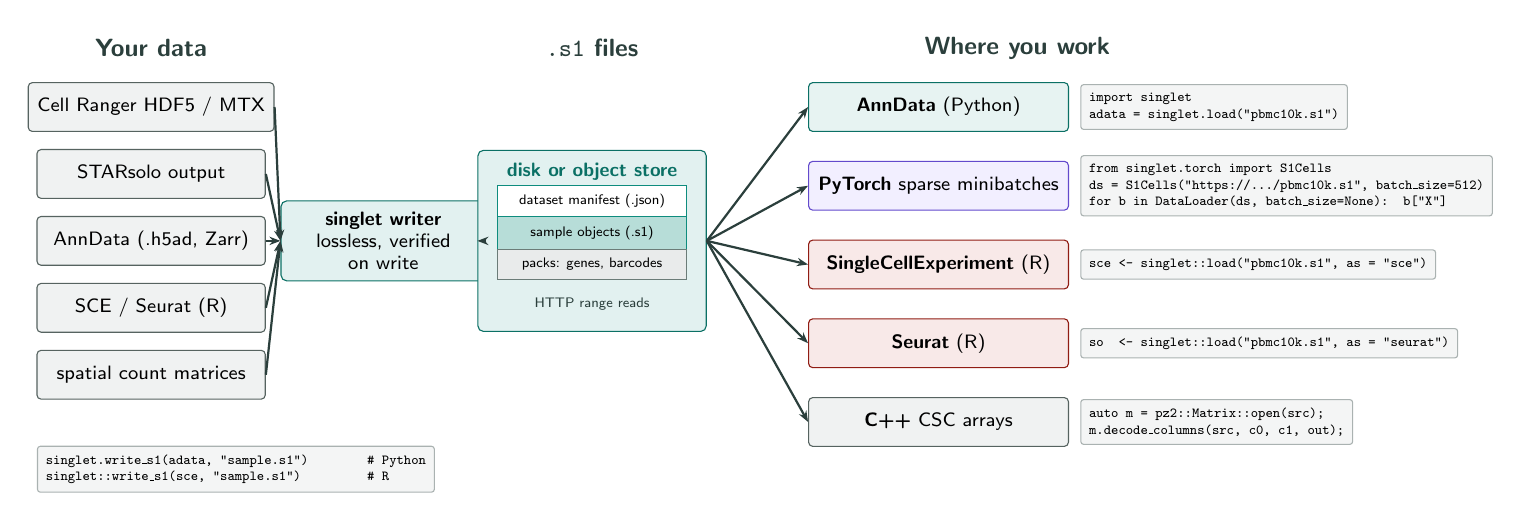
\begin{tikzpicture}[
  font=\sffamily\scriptsize,
  src/.style={draw=gen!80!black, fill=gen!10, rounded corners=1.5pt, minimum width=2.9cm, minimum height=0.62cm, align=center},
  hub/.style={draw=sone!80!black, fill=sone!12, rounded corners=2pt, align=center, inner sep=4pt},
  out/.style={draw=#1!80!black, fill=#1!10, rounded corners=1.5pt, minimum width=3.3cm, minimum height=0.62cm, align=center},
  code/.style={draw=ink2!40, fill=ink2!5, rounded corners=1pt, align=left, inner sep=3pt, font=\ttfamily\tiny, anchor=west},
  arr/.style={-{Stealth[length=4pt]}, thick, ink2},
  hdr/.style={font=\sffamily\small\bfseries, text=ink2},
]
% ---------- column headers ----------
\node[hdr] at (0,0.75) {Your data};
\node[hdr] at (5.6,0.75) {\sone{} files};
\node[hdr] at (11.0,0.75) {Where you work};

% ---------- sources ----------
\node[src] (cr) at (0,0)     {Cell Ranger HDF5 / MTX};
\node[src] (ss) at (0,-0.85) {STARsolo output};
\node[src] (ad) at (0,-1.7)  {AnnData (.h5ad, Zarr)};
\node[src] (sr) at (0,-2.55) {SCE / Seurat (R)};
\node[src] (sp) at (0,-3.4)  {spatial count matrices};

% ---------- writer ----------
\node[hub, minimum width=2.6cm] (wr) at (2.95,-1.7) {\textbf{singlet writer}\\lossless, verified\\on write};
\foreach \s in {cr,ss,ad,sr,sp} \draw[arr] (\s.east) -- (wr.west);

% ---------- the objects ----------
\node[hub, minimum width=2.9cm, minimum height=2.3cm] (obj) at (5.6,-1.7) {};
\node[font=\sffamily\scriptsize\bfseries, text=sone!80!black] at (5.6,-0.82) {disk or object store};
\node[draw=sone, fill=white, minimum width=2.4cm, font=\sffamily\tiny] at (5.6,-1.2) {dataset manifest (.json)};
\node[draw=sone, fill=sone!30, minimum width=2.4cm, font=\sffamily\tiny] at (5.6,-1.6) {sample objects (.s1)};
\node[draw=gen, fill=gen!15, minimum width=2.4cm, font=\sffamily\tiny] at (5.6,-2.0) {packs: genes, barcodes};
\node[font=\sffamily\tiny, text=ink2] at (5.6,-2.5) {HTTP range reads};
\draw[arr] (wr.east) -- (obj.west);

% ---------- readers ----------
\node[out=sone] (py)  at (10.0,0.0)  {\textbf{AnnData} (Python)};
\node[out=tens] (pt)  at (10.0,-1.0) {\textbf{PyTorch} sparse minibatches};
\node[out=dl]   (sce) at (10.0,-2.0) {\textbf{SingleCellExperiment} (R)};
\node[out=dl]   (seu) at (10.0,-3.0) {\textbf{Seurat} (R)};
\node[out=gen]  (cpp) at (10.0,-4.0) {\textbf{C++} CSC arrays};
\foreach \o in {py,pt,sce,seu,cpp} \draw[arr] (obj.east) -- (\o.west);

% ---------- code beside each reader ----------
\node[code] at (11.8,0.0)  {import singlet\\adata = singlet.load("pbmc10k.s1")};
\node[code] at (11.8,-1.0) {from singlet.torch import S1Cells\\ds = S1Cells("https://.../pbmc10k.s1", batch\_size=512)\\for b in DataLoader(ds, batch\_size=None): b["X"]};
\node[code] at (11.8,-2.0) {sce <- singlet::load("pbmc10k.s1", as = "sce")};
\node[code] at (11.8,-3.0) {so \ <- singlet::load("pbmc10k.s1", as = "seurat")};
\node[code] at (11.8,-4.0) {auto m = pz2::Matrix::open(src);\\m.decode\_columns(src, c0, c1, out);};

% ---------- writer calls ----------
\node[code] at (-1.45,-4.6) {singlet.write\_s1(adata, "sample.s1")\ \ \ \ \ \ \ \ \# Python\\singlet::write\_s1(sce, "sample.s1")\ \ \ \ \ \ \ \ \ \# R};
\end{tikzpicture}}
\caption{\textbf{\sone{} in the single-cell ecosystem.} Count matrices from Cell Ranger, STARsolo, AnnData,
SingleCellExperiment, Seurat or spatial pipelines are written once as \sone{} files, and the writer checks that the file
decodes to exactly the input. The \texttt{singlet} package reads them into AnnData, PyTorch minibatches,
SingleCellExperiment, Seurat or plain C++ arrays, from a local file or by HTTP range requests. The code beside each
target is the complete call (\texttt{DataLoader} is PyTorch's); Table~\ref{tab:eco} gives the time each takes on two
benchmark datasets. All calls are in \texttt{singlet}~\nm{rel-singlet_py} (Python) and \nm{rel-singlet_r} (R).}
\label{fig:eco}
\end{figure*}


% Discussion. Interpretation, limitations and outlook; every number is \nm{key} from generated/numbers.tex.
\section{Discussion}
\label{sec:discussion}

A count matrix has been treated as a generic array: stored as coordinates or compressed columns, then handed to a
byte-level compressor that cannot see what the bytes mean. \sone{} instead codes what is known about counts. Most
non-zeros are ones; a cell's depth sets the rate of every gene in it; and genes ranked by how many cells express them
turn a cell's non-zeros into short gaps. With these regularities as contexts for a static entropy coder, the files are
\nm{ratio-h5ad_gzip}$\times$ smaller than gzip-compressed AnnData and \nm{ratioBestOther}$\times$ smaller than the most
compact general-purpose alternative, and they decode faster than any other format we measured, including uncompressed
arrays. The payload ladder (Fig.~\ref{fig:floor}a) shows where the gain comes from: a strong general-purpose compressor
applied to well-separated gap and value streams stops at \nm{ladder-L3_gaps_leb_zstd19} bits per non-zero, and the last
step to \nm{ladder-L4_s1_payload} comes from modelling, not from a better back-end coder. Genomic read formats learned
the same lesson~\cite{bonfield2022cram,numanagic2016comparison}.

\paragraph{Where the bytes are read.}
Size matters most where data move over a network. Atlases serve count matrices to thousands of users, and models that
train on them read every cell many times. A format that is both small and fast to decode moves the bottleneck back to the
model. Size alone is not the whole story, though: on a link with realistic latency, the number of round trips matters as
much as the number of bytes. The index at the head of every \sone{} member lets a reader plan all of a minibatch's
requests before sending any, and sending them together cut the time to a first minibatch by about
\nm{concurrency-gain-first}$\times$ on a 30\,ms link. The same plan-then-fetch pattern applies to any reader of
independently addressable chunks, and the \texttt{singlet} readers for atlas samples and for R use it as well.

\paragraph{How much is left.}
Cross-validated count models, including negative binomial and cluster-conditioned models, code the matrices a median of
\nm{s1AboveFloorPct}\% more compactly than \sone, and they are charged nothing for describing themselves. On read-count
protocols \sone{} codes the matrix more compactly than every model we fitted (Table~\ref{tab:floor}). The sampling bound
explains why the margin is small: about \nm{samplingPctMedian}\% of the \sone{} code length is the multinomial sampling
of molecules, which no lossless decoder can avoid. Knowing a cell's cluster is worth \nm{sharedBpnMedian} bits per
non-zero before the cost of the model. Larger gains therefore require giving up losslessness, for example by
quantising counts, or storing a model of the data rather than the data. Neither is acceptable for a primary archive,
and the second is outside the scope of a storage format.

\paragraph{Limitations.}
\begin{itemize}\itemsep 1pt
\item \emph{Hardware.} All timings come from \nm{threadsHeadline}--8 cores of shared cluster nodes of one type, with one of
  our timed jobs per node and other users' jobs beside it. Absolute rates depend on the CPU and disk; the comparisons
  between formats, measured on the same node and file, are what the conclusions rest on. On this CPU the AVX-512
  kernel gives no gain over AVX2.
\item \emph{Large matrices.} Above $4\times10^8$ non-zeros we timed a subset of formats, at one thread count and from
  local disk only. The R formats, RDS and BPCells, are not applicable above $2^{31}-1$ non-zeros, because an R
  \texttt{dgCMatrix} cannot hold such a matrix in memory. One planned dataset, a genome-wide Perturb-seq screen with
  6.3 billion non-zeros, was excluded because writing the comparison formats needed more memory and time than the
  campaign allowed.
\item \emph{Network tiers.} The network tiers are a local object store with a limit on total bandwidth and added
  latency; real object stores add variable latency and request costs. The 10\,Gbit/s tier exceeds what the test setup
  delivers and is flagged in the tables.
\item \emph{Scope.} \sone{} stores non-negative integer counts below $2^{32}$. Normalised or otherwise non-integer
  matrices are rejected, not rounded. Files are immutable; adding cells means writing a new sample object.
\item \emph{Writing.} We did not time writing. The \sone{} writer counts its tables in one pass over the matrix and then
  codes it, but the formats differ in how much writing costs.
\end{itemize}

\paragraph{Beyond single cells.}
Two out-of-domain count matrices, bulk RNA-seq gene counts and a bag-of-words corpus, were run as an extension. There
\sone{} is \nm{ext-gtex_bulk-ratio-h5ad_gzip}$\times$ and \nm{ext-nytimes_bow-ratio-h5ad_gzip}$\times$ smaller than
gzip-compressed AnnData. The same structure, heavy-tailed rank-frequency laws and many small counts, is what the codec
exploits, so any sparse count matrix of this kind can be stored the same way.


\section*{Data and code availability}
All datasets are public; accessions, file names, licences and SHA-256 checksums are in \texttt{datasets.yaml} and
Supplementary Table~\ref{S-tab:datasets}. The \sone{} codec, its Python, R and C++ interfaces (\texttt{singlet}
\nm{rel-singlet_py} for Python and \nm{rel-singlet_r} for R, \url{https://github.com/Singlet-Bio/singlet}), and the
benchmark pipeline that produces every figure, table and number in this paper
(\texttt{papers/manuscripts/s1-format/bench}) are open source under the MIT license, with the per-stage results behind the
figures in \texttt{papers/manuscripts/s1-format/results}. The supplementary material and the format specification are
provided as separate files.

\section*{Acknowledgments}
Computations ran on the Clipper cluster at Grand Valley State University; the author thanks the GVSU HPC team for their
support. This work received no specific funding. Claude (Anthropic), a large language model, was used as a coding assistant
to develop the \sone{} codec and the benchmark pipeline, and to draft and revise the text of this article and its
supplement. Every codec change was kept only if measured on real matrices and reproduced its input exactly; all results are
produced by the open pipeline, and the author reviewed and takes responsibility for all content.

\bibliographystyle{IEEEtran}
\bibliography{refs}
\end{document}
